% §7 Implementation --- blueprint chapter 14 (blueprint/src/parts/14-implementation.tex),
% statements and proofs of record verbatim. Drafted 2026-09-15. The chapter has no Lean
% scheduled (as the causal article's implementation chapter has none); section 1.1 says so, and
% the body no longer does. Prose rewritten 2026-09-18 at the author's review
% (scripts/splice-prose.py, the statements and proofs untouched): a head that starts from how a
% scale space is computed in practice and says why nothing in the scale direction needs
% approximating, a numbered map of the four statements, four subsections each opening with its
% motivation, the technical notes on the index of the profile sum and on the quadrature weights
% moved after their statements, "pyramid" introduced where it is first used, and a block
% diagram of the cascade and of one Matern stage (fig-sections.tex). The map's item on rational
% increments states one direction only; the converse is rem:rational-converse's expectation.
%
% Contents and departures from the blueprint chapter:
%   - all four statement nodes transcribed under their markers: prop:knot-exactness,
%     prop:matern-cascade, prop:rational-increments, prop:thorin-machine;
%   - rem:recursive-gaussians, rem:rational-converse, rem:cannot-march and rem:costs are
%     copied; rem:cannot-march's two references into the locality and non-creation chapters
%     (module C, unreleased) are replaced by a sentence naming the next module's subject with
%     no statement number and no promise (hub RELEASES.md rule 1; CLAUDE.md: never by section
%     number of another deliverable); rem:recursive-gaussians names the two classical filter
%     families since 2026-09-19 (R174), their pole structure having been read from held copies
%     on 2026-09-18, and gives its infinite-divisibility criterion a pointer, so the blueprint's
%     CHECK on that literature is discharged and is gone from both files;
%   - the chapter's opening paragraph is this section's relation-to-the-causal-theory
%     sentence (ADR-0003); no further causal remark;
%   - the paragraph after prop:thorin-machine on the spectra of the working families is kept.

\section{Implementation: exact cascades and recursive sections}\label{sec:implementation}

A scale-space representation is computed at finitely many scales, and the usual way to compute
it is to treat each scale separately: convolve the signal with the kernel of that scale,
truncated to a finite filter, or replace the kernel by a recursive filter that approximates
it (\sscite{deriche1993recursively,young1995recursive}). Both are approximations of the kernel. The discretization of the signal has a theory of
its own (\sscite{lindeberg1990scalespace}), and this section does not enter it: the statements
below are for signals on the line, and sampling the signal is a separate approximation. This
section is about the scale direction: for an admissible family nothing in that direction has
to be approximated. The family is a cascade. The record at one scale, the smoothed signal
there, is obtained from the record at the
previous scale by one stage, and the hemigroup axiom says that the result is the scale space
itself. So the axiom that defines the class is also its
algorithm, and what has to be implemented is a stage.

The section follows that thought, and Figure~\ref{fig:sections} is the picture. The cascade
reproduces the scale space exactly at every knot of any finite ladder of scales
(\S\ref{sec:knots}, Proposition~\ref{prop:knot-exactness}). For the \Matern{} family with
integer index a stage is a rational filter, realized by first-order recursive sections run
forward and backward along the signal, with positive coefficients and a cost per sample that
does not depend on the scale (\S\ref{sec:matern-cascade},
Proposition~\ref{prop:matern-cascade}), and a criterion on the pole--zero diagram says which
rational filters --- among them the recursive filters used for the Gaussian --- are themselves
scale spaces (Proposition~\ref{prop:rational-criterion},
Remark~\ref{rem:recursive-gaussians}). Finite
mixtures of \Matern{} members with integer weights have such stages too, a rational filter
generates a ladder of scales and one candidate family between its levels, and a family with
rational stages need not be of either kind (\S\ref{sec:rational},
Proposition~\ref{prop:rational-increments}, Remark~\ref{rem:rational-converse}). Every member
with a completely monotone profile is a limit of members with finitely many ranges, but the
families realized by the first-order sections reach only the members whose Thorin measure
consists of atoms of even integer mass, possibly with a Gaussian part, and so neither the
stable nor the Student-t members, which lack moments that every such limit has
(\S\ref{sec:thorin-machine}, Propositions~\ref{prop:thorin-machine}
and~\ref{prop:rational-closure}). \S\ref{sec:costs} collects the costs, and
\S\ref{sec:numerical-run} runs the cascade on a sampled signal, checks the statements on it,
and applies the criterion of Proposition~\ref{prop:rational-criterion} to two published
recursive Gaussians
(Example~\ref{ex:numerical-run}).
The causal theory has the same structure on the time axis, with one-sided first-order
sections (\sscite{fagerstrom2026hemigroup}). What is new on the line is that a section becomes
a forward--backward pair, the form of recursive filter that image processing has long used for
the Gaussian, and that the theory says which of those filters are scale spaces.

% Figure: the cascade over a knot ladder, and one Matern stage as forward and backward
% first-order sections. Referenced from section 7. Pure TikZ, schematic (2026-09-18, the
% author's review). Top: the knot ladder, exact at every knot (prop:knot-exactness). Bottom:
% one stage for integer gamma (prop:matern-cascade).

\begin{figure}[t]
\centering
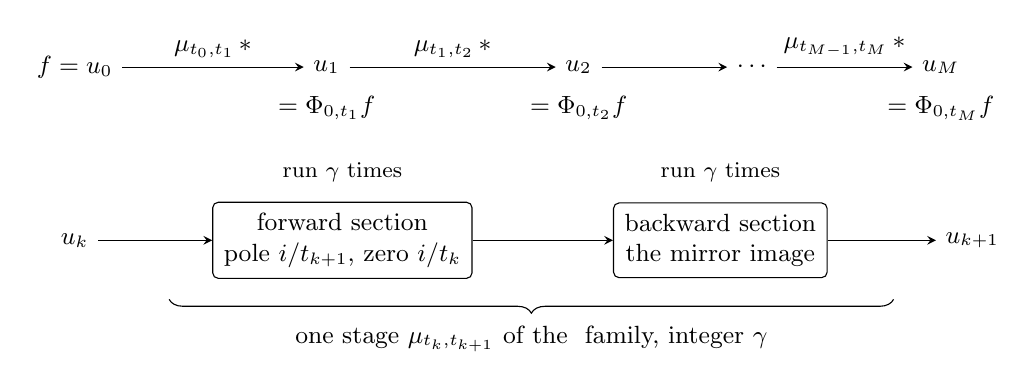
\begin{tikzpicture}[every node/.style={font=\small}, >=stealth,
  box/.style={draw, rounded corners=2pt, minimum height=8mm, inner sep=4pt, align=center}]

% --- the knot ladder ------------------------------------------------------------------------
\node (u0) at (0,2.2) {$f = u_0$};
\node (u1) at (3.2,2.2) {$u_1$};
\node (u2) at (6.4,2.2) {$u_2$};
\node (ud) at (8.6,2.2) {$\cdots$};
\node (uM) at (11.0,2.2) {$u_M$};
\draw[->] (u0) -- node[above] {$\mu_{t_0,t_1}\,*$} (u1);
\draw[->] (u1) -- node[above] {$\mu_{t_1,t_2}\,*$} (u2);
\draw[->] (u2) -- (ud);
\draw[->] (ud) -- node[above] {$\mu_{t_{M-1},t_M}\,*$} (uM);
\node[anchor=north] at (3.2,1.95) {$= \Phi_{0,t_1}f$};
\node[anchor=north] at (6.4,1.95) {$= \Phi_{0,t_2}f$};
\node[anchor=north] at (11.0,1.95) {$= \Phi_{0,t_M}f$};

% --- one Matern stage -----------------------------------------------------------------------
\node (in) at (0,0) {$u_k$};
\node[box] (fw) at (3.4,0) {forward section\\ pole $i/t_{k+1}$, zero $i/t_k$};
\node[box] (bw) at (8.2,0) {backward section\\ the mirror image};
\node (out) at (11.4,0) {$u_{k+1}$};
\draw[->] (in) -- (fw);
\draw[->] (fw) -- (bw);
\draw[->] (bw) -- (out);
\node[anchor=south] at (3.4,0.62) {\footnotesize run $\gamma$ times};
\node[anchor=south] at (8.2,0.62) {\footnotesize run $\gamma$ times};
\draw[decorate, decoration={brace, amplitude=5pt, mirror}] (1.2,-0.75) -- (10.4,-0.75)
  node[midway, below=6pt] {one stage $\mu_{t_k,t_{k+1}}$ of the \Matern{} family, integer $\gamma$};

\end{tikzpicture}
\caption{The cascade as an algorithm. Top: over any ladder of scale knots the cascade of
stages reproduces the scale space exactly at every knot
(Proposition~\ref{prop:knot-exactness}). Bottom: for the \Matern{} family with integer
$\gamma$, a stage is $\gamma$ first-order recursive sections run forward along the signal
followed by $\gamma$ run backward (the label above a box says how often its section is run), each with
one state and with positive coefficients
(Proposition~\ref{prop:matern-cascade}).}
\label{fig:sections}
\end{figure}


\subsection{Exactness at the knots}\label{sec:knots}

Choose the scales at which the representation is wanted, $0 = t_0 < t_1 < \dots < t_M$, start
from the signal, and compute each record from the previous one. The proposition says that
this computes the scale space, and that adding knots later changes nothing at the old ones.

% shared with blueprint prop:knot-exactness
\begin{proposition}[exactness at the knots]\label{prop:knot-exactness}
Let $0 = t_0 < t_1 < \dots < t_M$ be any finite set of scale knots and define the discrete
cascade $u_0 := f$, $u_{k+1} := \mu_{t_k,t_{k+1}} * u_k$. Then $u_k = \Phi_{0,t_k}f$ exactly for
every $k$, and refining the knot set changes nothing at the old knots. On the transform side the
increment transforms telescope,
$\prod_{k<M} e^{-F(t_{k+1}\omega) + F(t_k\omega)} = e^{-F(t_M\omega)}$.
\end{proposition}

The cascade is the family sampled at the knots, so there is no discretization error in scale
to control. Since the family exists at every scale, a ladder of knots can also be shifted at will,
and an arbitrary dilation is handled by instantiating the family at the shifted knots.

\begin{proof}
Induction on (A6): $\mu_{0,t_{k+1}} = \mu_{t_k,t_{k+1}} * \mu_{0,t_k}$, by
Lemma~\ref{lem:additivity}, and $u_0 = \Phi_{0,t_0}f = f$.
\end{proof}

\subsection{The \texorpdfstring{\Matern{}}{Matern} cascade}\label{sec:matern-cascade}

Exactness at the knots is useful only if a stage can be computed, and in general a stage is a
convolution with a kernel that has no closed form. The \Matern{} family with integer index is
the case where a stage costs one state and a few operations per sample. The transform of a
stage is a ratio of two polynomials in $\omega^2$ of the same degree, and each of its factors
splits into a part with its pole in the upper half-plane and a part with its pole in the lower
one. The first is a causal first-order recursive filter along the signal, a \emph{lag section} as
the proposition names it, and the second is its mirror image. Running the one forward and the
other backward realizes their product, which is the symmetric stage. Each section is a convex
combination of the identity and a one-sided exponential average, so positivity and unit mass
hold already at the level of the realization.

% shared with blueprint prop:matern-cascade
\begin{proposition}[the \Matern{} cascade: forward--backward first-order sections]
\label{prop:matern-cascade}
For the \Matern{} family with integer $\gamma$, so that $e^{-F(t\omega)} =
(1+t^2\omega^2)^{-\gamma}$, the increment between adjacent knots has transform
\begin{equation}\label{eq:matern-increment}
  \hat\mu_{t_k,t_{k+1}}(\omega)
  = \Bigl(\frac{1 + t_k^2\omega^2}{1 + t_{k+1}^2\omega^2}\Bigr)^{\gamma}
  = \Bigl(\frac{1 + it_k\omega}{1 + it_{k+1}\omega}\cdot
          \frac{1 - it_k\omega}{1 - it_{k+1}\omega}\Bigr)^{\gamma},
\end{equation}
a cascade of $\gamma$ identical causal first-order pole--zero sections in $x$, called \emph{lag
sections} below, and $\gamma$ identical anticausal ones, each with the one-state realization
\[
  w' = \frac{y - w}{t_{k+1}} \quad(\text{forward}),
  \qquad
  v = \frac{t_k}{t_{k+1}}\,y + \Bigl(1 - \frac{t_k}{t_{k+1}}\Bigr) w,
\]
and its mirror image run backward. Which solution of the state equation is meant is part of the
realization: its solutions differ by a multiple of $e^{-x/t_{k+1}}$, and the one intended is the
solution in $\Lone$, equivalently the one with $w(-\infty) = 0$ for the forward pass and
$w(+\infty) = 0$ for the backward one. The zero of the transfer function costs no differentiation of
the input: the output is a convex combination of the input and the state. The section's kernel is
the mixture
$\tfrac{t_k}{t_{k+1}}\delta_0 + (1 - \tfrac{t_k}{t_{k+1}})\,\Expo_{+}(t_{k+1})$ of no
displacement and a one-sided exponential displacement, $\Expo_{\pm}(t)$ denoting the one-sided
exponential kernels $t^{-1}e^{-|x|/t}$ carried by $\pm(0,\infty)$; so the two-sided increment for
$\gamma = 1$ is the four-term mixture
\begin{equation}\label{eq:four-term}
  r^2\,\delta_0 + r(1-r)\bigl(\Expo_+ + \Expo_-\bigr) + (1-r)^2\,\Lap_{t_{k+1}},
  \qquad r := \frac{t_k}{t_{k+1}} \in (0,1),
\end{equation}
where $\Expo_\pm$ are taken at the range $t_{k+1}$ and $\Lap_t$ is the Laplace kernel of range
$t$; positivity and unit mass are manifest at the
realization level. Sampled on a grid, a full scale space over $M$ knots costs $2\gamma M$
first-order states and $O(\gamma M)$ multiply--adds per sample, in a forward and a backward pass
\emph{at each knot}. Sampling the signal
is a separate approximation and is not treated here.
\end{proposition}

\begin{proof}
The increment transform is the ratio of the endpoint transforms, the denominators being
nonvanishing (Lemma~\ref{lem:nonvanishing}), which is
Proposition~\ref{prop:matern-exponent}(2); the factorization is
$1 + t^2\omega^2 = (1+it\omega)(1-it\omega)$. The transfer identity of the section is
\[
  \frac{t_k}{t_{k+1}} + \Bigl(1 - \frac{t_k}{t_{k+1}}\Bigr)\frac{1}{1+it_{k+1}\omega}
  = \frac{1 + it_k\omega}{1 + it_{k+1}\omega},
\]
and the convex-combination clause is $0 < t_k/t_{k+1} < 1$. In particular the output is a convex
combination of the input and the state, so the section differentiates nothing. For
\ref{eq:four-term}, convolve the
causal and anticausal mixtures and use $\Expo_+(t) * \Expo_-(t) = \Lap_t$, whose transform identity
is $(1+it\omega)^{-1}(1-it\omega)^{-1} = (1+t^2\omega^2)^{-1}$.
\end{proof}

The proposition bears on the approximation of the Gaussian by recursive filters, and it turns
into a test. A recursive filter is given by its transfer function, which is a rational function
of $\omega$; the question is whether that function is the transform of the kernel of an
admissible family, in which case the filter is not an approximation of a scale space but a scale
space. The next proposition answers it from the pole--zero diagram alone, in three conditions.
The first is a glance at the real axis. The other two are read off one explicit exponential sum,
built by giving every pole a positive exponential term and every zero a negative one: that sum is
the candidate profile, and the filter is a scale space exactly when it is a profile at all,
nonnegative and nonincreasing. Example~\ref{ex:numerical-run} applies the test to two published
designs.

% shared with blueprint prop:rational-criterion
\begin{proposition}[which rational transfer functions are admissible kernels]
\label{prop:rational-criterion}
Let $R$ be an even rational function with $R(0) = 1$, written in lowest terms. Write
$\pm i\theta_1,\dots,\pm i\theta_M$ for its poles and $\pm i\zeta_1,\dots,\pm i\zeta_L$ for its
zeros, listed with multiplicity and normalised by $\Rea\theta_m > 0$ and $\Rea\zeta_l > 0$; both
lists are closed under conjugation, so the \emph{signed profile}
\begin{equation}\label{eq:rational-profile}
  k(x) \ :=\ 2\sum_{m \le M} e^{-\theta_m x} \ -\ 2\sum_{l \le L} e^{-\zeta_l x},
  \qquad x > 0,
\end{equation}
is real-valued. Then $R$ is the transform of the kernel at canonical scale $1$ of an admissible
family --- equivalently, $-\log R$ is an admissible exponent --- if and only if
\begin{enumerate}
\item $R$ has neither a pole nor a zero on the real axis, so that $R > 0$ there;
\item $k \ge 0$ on $(0,\infty)$; and
\item $k$ is nonincreasing on $(0,\infty)$.
\end{enumerate}
The family is then the one with Gaussian coefficient $0$ and folded profile $k$. Condition (i)
alone excludes every $R$ with a real zero, since the transform of an infinitely divisible law has
no zero at all (Lemma~\ref{lem:nonvanishing}).
\end{proposition}

A Gaussian factor is not covered and needs none: a rational $R$ forces the Gaussian coefficient
to vanish, which is the growth argument in the proof, and a design with a Gaussian factor is that
factor times a rational one. The criterion is for the transfer function on the line; a sampled
filter is a different object, and the discrete classification is a different theory
(\sscite{lindeberg1990scalespace}).

\begin{proof}
\emph{The factorisation.} $R$ is even and rational, so $R(\omega) = N(\omega^2)/D(\omega^2)$ for
polynomials $N$ and $D$ with no common factor, real because $R$ is real on the real axis. Its
poles and zeros are therefore closed under $\omega \mapsto -\omega$ and under conjugation, and
under (i) none of them is real; choosing from each pair $\pm\omega_0$ the one in the upper
half-plane and writing it as $i\theta$ with $\Rea\theta > 0$ gives the two lists of the statement,
each closed under conjugation. Then $D(\omega^2) = c_D\prod_m(\omega^2+\theta_m^2)$ and
$N(\omega^2) = c_N\prod_l(\omega^2+\zeta_l^2)$, and $R(0) = 1$ fixes the constant:
\begin{equation}\label{eq:rational-factored}
  R(\omega) \ =\ \frac{\prod_{l \le L}\bigl(1 + \omega^2/\zeta_l^2\bigr)}
                      {\prod_{m \le M}\bigl(1 + \omega^2/\theta_m^2\bigr)} .
\end{equation}

\emph{The exponential-profile identity at a complex rate.} For $\Rea\theta > 0$ and $\omega$ real,
\begin{equation}\label{eq:complex-frullani}
  \int_0^\infty \bigl(1 - \cos\omega x\bigr)\,e^{-\theta x}\,\frac{dx}{x}
   \ =\ \tfrac12\bigl[\Log(\theta - i\omega) + \Log(\theta + i\omega)\bigr] - \Log\theta ,
\end{equation}
with $\Log$ the principal logarithm, which is what Proposition~\ref{prop:matern-exponent}(1) says
at a real rate. Indeed $1 - \cos\omega x = 1 - \tfrac12(e^{i\omega x} + e^{-i\omega x})$, so the
integral is half the sum of $\int_0^\infty(e^{-\theta x} - e^{-(\theta \mp i\omega)x})\,dx/x$, and
for two points $\alpha,\beta$ of the open right half-plane
\[
  \int_0^\infty \bigl(e^{-\alpha x} - e^{-\beta x}\bigr)\frac{dx}{x}
   = \int_0^\infty\!\!\int_{[\alpha,\beta]} e^{-sx}\,ds\,dx
   = \int_{[\alpha,\beta]}\frac{ds}{s} = \Log\beta - \Log\alpha ,
\]
the segment $[\alpha,\beta]$ lying in that half-plane by convexity: the exchange is Fubini, the
modulus of the inner integrand being at most $e^{-cx}$ with $c > 0$ the least real part on the
segment, which is integrable against $dx$ on $[1,\infty)$ while on $(0,1)$ the inner integral is
bounded by $|\beta - \alpha|$; and $1/s$ is analytic on a neighbourhood of the segment, where
$\Log$ is a primitive.

\emph{The exponent of the signed profile.} $k$ of \ref{eq:rational-profile} is continuous on
$(0,\infty)$, bounded there by $2(M+L)$, and $|k(x)| \le 2(M+L)e^{-cx}$ with
$c := \min_m\Rea\theta_m \wedge \min_l\Rea\zeta_l > 0$; so
$\int_0^\infty(1-\cos\omega x)|k(x)|\,dx/x$ is finite, the integrand being $O(x)$ at the origin
and exponentially small at infinity. Summing \ref{eq:complex-frullani} over the two lists,
\[
  \Psi(\omega) \ :=\ \int_0^\infty \bigl(1 - \cos\omega x\bigr)\,k(x)\,\frac{dx}{x}
   \ =\ \sum_{m}\Log\Bigl(1 + \frac{\omega^2}{\theta_m^2}\Bigr)
        - \sum_{l}\Log\Bigl(1 + \frac{\omega^2}{\zeta_l^2}\Bigr) ,
\]
where each summand is $\Log(\theta-i\omega) + \Log(\theta+i\omega) - 2\Log\theta$ and no branch is
chosen for a product: the value is real, since conjugate rates contribute conjugate summands and a
real rate a real one. Exponentiating kills the branches, $e^{\Log z} = z$ for every $z \ne 0$, and
\ref{eq:rational-factored} gives $e^{-\Psi(\omega)} = R(\omega)$. So $\Psi = -\log R$ with the
real logarithm of a positive number, at every real $\omega$.

\emph{Sufficiency.} Assume (i), (ii) and (iii). Then $k$ is nonnegative, nonincreasing, bounded on
$(0,1]$ and exponentially small at infinity, so $\int_0^1 x\,k(x)\,dx$ and
$\int_1^\infty k(x)\,x^{-1}dx$ are finite: by Lemma~\ref{lem:profile-integrability} the pair
$(0,k)$ is of the form \ref{eq:sd-profile}, and by Theorem~\ref{thm:main-characterization} it is
the pair of an admissible family, whose exponent is $\Psi = -\log R$. The transform of its kernel
at canonical scale $1$ is $e^{-\Psi} = R$.

\emph{Necessity.} Assume $R = e^{-F}$ with $F$ admissible, of data $(a,k_F)$. Then $R > 0$ and
$R \le 1$ on the real axis, so $R$ has there neither a zero nor a pole, which is (i). Next
$a = 0$: by \ref{eq:rational-factored} $|R(\omega)|$ is bounded above and below by multiples of
$|\omega|^{2(L-M)}$ for large $|\omega|$, so $F = -\log R$ grows at most like a multiple of
$\log|\omega|$, while $F(\omega) \ge a\omega^2$ for every $\omega$. So $F = \Psi$ by the previous
paragraph, that is
\[
  \int_0^\infty (1 - \cos\omega x)\,k_F(x)\,\frac{dx}{x}
   = \int_0^\infty (1 - \cos\omega x)\,k(x)\,\frac{dx}{x}, \qquad \omega \in \RR ,
\]
an identity between an exponent with a positive \Levy{} measure and one with a signed density.
The uniqueness of the \Levy{} pair (Proposition~\ref{prop:fourier-toolbox}(3)) is stated for
positive measures, so it is applied after a recombination, as in the proof of
Lemma~\ref{lem:cin-delay-equation}: writing $k = k^{+} - k^{-}$ for the positive and negative
parts, both $(k_F + k^{-})(x)\,dx/x$ and $k^{+}(x)\,dx/x$ are positive measures on $(0,\infty)$
satisfying the \Levy{} condition --- each of $k^{\pm}$ is dominated by $|k|$, which does --- and
the displayed identity says that the two pairs $(0,(k_F+k^{-})\,dx/x)$ and $(0,k^{+}\,dx/x)$ have
the same exponent. Hence they are equal, and $k_F = k$ almost everywhere on $(0,\infty)$. Since
$k$ is continuous and $k_F$ is nonnegative and nonincreasing, the identity holds everywhere and
$k$ inherits both properties: the agreement set is conull, hence meets every interval, and
approaching a given $x$ from each side through it gives $k(x) \ge k(y)$ for $x < y$ and
$k \ge 0$. That is (ii) and (iii).

\emph{The last sentence.} If $R$ vanishes at a real $\omega_0$ then $R$ is the transform of no
infinitely divisible law, the transform of such a law having no zero
(Lemma~\ref{lem:nonvanishing}); in particular it is the transform of no admissible kernel.
\end{proof}

% blueprint rem:recursive-gaussians, copied (the short form of 2026-09-19, R198)
\begin{remark}[which recursive Gaussians are scale spaces]
\label{rem:recursive-gaussians}
Read at the designs of the image-processing literature, the criterion says the following. If the
transfer has only real poles and no zeros, then $R = \prod_i(1+t_i^2\omega^2)^{-1}$, whose signed
profile $2\sum_ie^{-x/t_i}$ is positive and decreasing, so the three conditions hold and the
filter is the kernel of the symmetric Thorin member with atoms at $1/t_i$
(Proposition~\ref{prop:thorin-subclass}), the multi-range \Matern{}; its dilates form a scale
space whose increments are again forward--backward lag sections. The classical all-pole
approximations of the Gaussian with real poles --- in particular the cascade of $\gamma$
identical first-order sections at $t = \sigma/\sqrt{2\gamma}$, whose transfer is
$(1+\sigma^2\omega^2/2\gamma)^{-\gamma} \to e^{-\sigma^2\omega^2/2}$ --- are therefore not
approximations of a scale space but scale spaces, \Matern{} members converging to the Gaussian
along $\gamma$ at matched variance, the variance being $2\gamma t^2$ by
Proposition~\ref{prop:matern-exponent}(3). Neither complex poles nor zeros off the real axis are
excluded in advance, and neither is harmless. A complex pair contributes a term
$e^{-cx}\cos(dx)$ to the signed profile, which changes sign by itself, so condition (ii) has to
be checked against the other terms; a real pole of sufficient weight can carry such a pair, and
Remark~\ref{rem:rational-converse} exhibits an admissible family that does, of exponent
$3\log(1+\omega^2) + \log(1+\omega^4/4)$. A zero of the transfer on the real axis fails (i)
outright, while a zero off it is a term subtracted in \ref{eq:rational-profile} and may leave
(ii) and (iii) standing or not: the second example of that remark, of exponent
$2\log(1+\omega^2) - \log(1+\omega^2/4)$, has all its poles and zeros on the imaginary axis, is
admissible, and is neither a Thorin member nor realized by lag sections. The two standard
recursive Gaussians of the image-processing literature are optimized for accuracy and are decided
by different conditions. The design of \sscite{deriche1993recursively} \emph{adds} a causal and an
anticausal half (\S5.1, (38), two complex-conjugate pole pairs), so its transfer is not a modulus
squared at all, and at the published coefficients that sum has zeros on the real axis: it fails
(i). The design of \sscite{young1995recursive} is a forward--backward cascade with one real pole
and one conjugate pair (p.~141, Table~1 with (6a)--(6b)); it passes (i), and at the published
coefficients its signed profile goes negative, so it fails (ii). Each verdict is a computation on
the printed coefficients of one design and not a theorem about a class of designs;
Example~\ref{ex:numerical-run} carries both out. Whatever their accuracy as Gaussian
approximations, a filter whose $R$ fails the test is the kernel of no exact cascade. The theory's
recommendation is therefore the opposite of the literature's optimization: approximate the
Gaussian \emph{from inside the class}, by real-pole cascades with no zeros, and accept the
\Matern{}'s exponential tails and its kink at the origin for $\gamma = 1$ as the price of
exactness in scale.
\end{remark}

\subsection{Rational increments and the pyramid they interpolate}\label{sec:rational}

Two questions follow. Which other families have rational stages, and what can be said of a
rational filter that is given in advance, as a recursive filter usually is? The first clause
of the proposition answers the first: a finite mixture of \Matern{} members with integer
weights $w_i$ in the exponent has rational stages of order $2\sum_i w_i$, realized by lag
sections as before. The
second clause starts from a single rational filter $R$ that is the transform of an infinitely
divisible law, and asks for a scale space in which $R$ is the stage between scales at a fixed
ratio $q$. Such a ladder of scales at ratio $q$, with covariance under dilation by $q$ alone,
is a \emph{pyramid} in the sense of multiresolution practice (\sscite{burt1983laplacian}). The
clause says that $R$ and $q$ determine one pyramid. They also determine one candidate for a
fully covariant family that interpolates the pyramid, and the candidate is admissible exactly
when its profile is nonincreasing. The \Matern{} pyramid is the case $R = (1+\omega^2)^{-1}$.
The family that interpolates it has the exponent $\sum_{m \ge 1}\log(1 + q^{-2m}\omega^2)$, a
mixture of \Matern{} members over the ranges $q^{-m}$, and it is a different member from the
\Matern{} family: its stages are rational only between scales at ratio $q^n$, whereas those of
the \Matern{} family are rational between every pair of scales. Figure~\ref{fig:pyramid} shows
the ladder, the family between its levels, and the profile of that family.

% Figure: the pyramid of prop:rational-increments(2) and the family that interpolates it.
% Referenced from section 7.3 before the proposition. Pure TikZ, schematic (2026-09-19, the
% author's review: a schematic of the pyramid). Left: the ladder of scales at ratio q, the same
% filter R dilated from level to level, and the interpolating family between the levels; the
% sample marks getting sparser by q per level are the subsampling of multiresolution practice,
% drawn for orientation only (the statement is on the line and involves no sampling). Right: the
% folded profile of the interpolating family of the Matern pyramid, R = 1/(1 + omega^2), q = 2,
% k(x) = 2 sum_{m >= 1} exp(-2^m x), against log_2 x; the coordinates were computed in Python
% (the sum to machine precision) and pasted, since pgfmath overflows on the inner exponentials.

\begin{figure}[t]
\centering
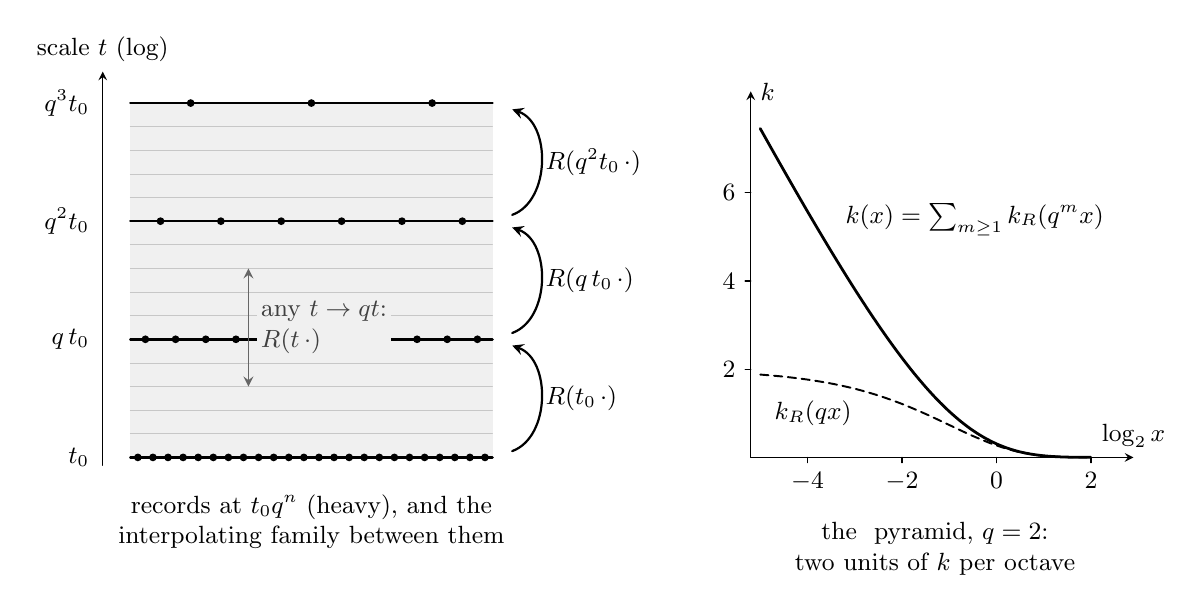
\begin{tikzpicture}[every node/.style={font=\small}, >=stealth, line cap=round]

% --- left: the ladder ---------------------------------------------------------------------
\begin{scope}[shift={(0,0)}]
\fill[black!6] (0,0) rectangle (4.6,4.5);
\foreach \y in {0.3,0.6,...,4.3} \draw[black!22, line width=0.3pt] (0,\y) -- (4.6,\y);
\draw[->] (-0.35,-0.1) -- (-0.35,4.9) node[above] {scale $t$ (log)};
\foreach \lev/\lab/\n in {0/{t_0}/24, 1.5/{q\,t_0}/12, 3.0/{q^2t_0}/6, 4.5/{q^3t_0}/3} {
  \draw[line width=0.9pt] (0,\lev) -- (4.6,\lev);
  \node[left] at (-0.4,\lev) {$\lab$};
  \pgfmathsetmacro{\step}{4.6/\n}
  \foreach \i in {1,...,\n} \fill ({(\i-0.5)*\step},\lev) circle (1.4pt);
}
\foreach \lo/\lab in {0/{R(t_0\,\cdot)}, 1.5/{R(q\,t_0\,\cdot)}, 3.0/{R(q^2t_0\,\cdot)}} {
  \draw[->, line width=0.8pt] (4.85,\lo+0.08) to[out=20,in=-20] (4.85,\lo+1.42);
  \node[right] at (5.15,\lo+0.75) {$\lab$};
}
\draw[<->, line width=0.6pt, black!60] (1.5,0.9) -- (1.5,2.4);
\node[right, black!75, align=left, fill=black!6, inner sep=1.5pt] at (1.6,1.65)
  {any $t \to qt$:\\ $R(t\,\cdot)$};
\node[anchor=north, align=center] at (2.3,-0.35)
  {records at $t_0q^n$ (heavy), and the\\ interpolating family between them};
\end{scope}

% --- right: the profile of the interpolating family ---------------------------------------
\begin{scope}[shift={(11.0,0)}, x=0.6cm, y=0.56cm]
\draw[->] (-5.2,0) -- (2.9,0) node[above] {$\log_2 x$};
\draw[->] (-5.2,0) -- (-5.2,8.3) node[right] {$k$};
\foreach \x in {-4,-2,0,2} \draw (\x,0) -- (\x,-0.12) node[below] {$\x$};
\foreach \y in {2,4,6} \draw (-5.2,\y) -- (-5.32,\y) node[left] {$\y$};
\draw[line width=1.0pt] plot[smooth] coordinates
 {(-5.000,7.458) (-4.750,6.981) (-4.500,6.509) (-4.250,6.041) (-4.000,5.579) (-3.750,5.125)
  (-3.500,4.678) (-3.250,4.241) (-3.000,3.814) (-2.750,3.401) (-2.500,3.002) (-2.250,2.620)
  (-2.000,2.257) (-1.750,1.915) (-1.500,1.598) (-1.250,1.306) (-1.000,1.044) (-0.750,0.812)
  (-0.500,0.611) (-0.250,0.444) (0.000,0.308) (0.250,0.203) (0.500,0.125) (0.750,0.072)
  (1.000,0.037) (1.250,0.017) (1.500,0.007) (1.750,0.002) (2.000,0.001)};
\draw[line width=0.7pt, densely dashed] plot[smooth] coordinates
 {(-5.000,1.879) (-4.500,1.831) (-4.000,1.765) (-3.500,1.676) (-3.000,1.558) (-2.500,1.404)
  (-2.000,1.213) (-1.500,0.986) (-1.000,0.736) (-0.500,0.486) (0.000,0.271) (0.500,0.118)
  (1.000,0.037) (1.500,0.007) (2.000,0.001)};
\node[right] at (-3.4,5.4) {$k(x) = \sum_{m \ge 1} k_R(q^mx)$};
\node[right] at (-4.9,1.0) {$k_R(qx)$};
\node[anchor=north, align=center] at (-1.3,-1.25)
  {the \Matern{} pyramid, $q = 2$:\\ two units of $k$ per octave};
\end{scope}
\end{tikzpicture}
\caption{The pyramid of Proposition~\ref{prop:rational-increments}(2), schematically. Left: a
ladder of scales at ratio $q$. The stage from one level to the next is one rational filter
$R$, dilated with the level, and the proposition gives the one family that has these stages
and exists at every scale between the levels. For that family the stage from any scale $t$ to
$qt$ is $R(t\,\cdot)$, so the ladder can start at any $t_0$. The marks on the levels,
sparser by $q$ from level to level, show the subsampling that a pyramid in multiresolution
practice adds to such a ladder. They are drawn for orientation: the statement is about
convolution ladders on the line and involves no subsampling. Right: the folded profile of the
interpolating family for $R = (1+\omega^2)^{-1}$ and $q = 2$, with its first term dashed. Each
level of the ladder adds one copy of $k_R$, dilated by $q$, so the profile grows by
$k_R(0{+}) = 2$ per octave as $x \to 0$ and is unbounded at the origin, where the profile
$2\gamma e^{-x}$ of a \Matern{} member is bounded.}
\label{fig:pyramid}
\end{figure}


% shared with blueprint prop:rational-increments
\begin{proposition}[rational increments and the pyramid they interpolate]
\label{prop:rational-increments}
\begin{enumerate}
\item If
\[
  F(\omega) = \sum_{i=1}^N w_i\log\Bigl(1 + \frac{\omega^2}{\theta_i^2}\Bigr)
\]
with positive integer weights $w_i$ and no Gaussian part, then every increment is rational,
\[
  \hat\mu_{s,t} = \prod_i\Bigl(\frac{1 + s^2\omega^2/\theta_i^2}{1 + t^2\omega^2/\theta_i^2}\Bigr)^{w_i},
\]
of order $2\sum_i w_i$, realized by $\sum_i w_i$ forward and $\sum_i w_i$ backward lag sections,
each pole--zero pair at the common ratio $s/t$.
\item Let $R$ be a symmetric rational function that is the transform of an infinitely divisible
law, with folded \Levy{} profile $k_R$. Then for each $q > 1$ there is exactly one function $F$
that is continuous with $F(0) = 0$ and satisfies $F(q\omega) - F(\omega) = -\log R(\omega)$,
namely
\[
  e^{-F(\omega)} = \prod_{m \ge 1} R\bigl(q^{-m}\omega\bigr),
  \qquad \text{with folded profile} \quad
  k(x) = \sum_{m \ge 1} k_R\bigl(q^m x\bigr);
\]
it is admissible exactly when this $k$ is nonincreasing, in particular whenever $k_R$ is. The
\Matern{} pyramid is the case $R(\omega) = (1+\omega^2)^{-1}$.
\end{enumerate}
\end{proposition}

The index in the profile sum runs from $m = 1$. Write $F = \sum_{m \ge 1}\psi(q^{-m}\,\cdot)$
with $\psi = -\log R$. The dilate $\psi(c\,\cdot)$ has profile $k_R(x/c)$, so the term with
$c = q^{-m}$ contributes $k_R(q^mx)$. An $m = 0$ term would make the $q$-step increment
$\psi(q\,\cdot)$ in place of $\psi$.

\begin{proof}
(1) The increment transform telescopes by Proposition~\ref{prop:knot-exactness}, and each
factor $\bigl((1+s^2\omega^2/\theta^2)/(1+t^2\omega^2/\theta^2)\bigr)$ is realized as in
Proposition~\ref{prop:matern-cascade} after the gauge change $t \mapsto t/\theta$;
admissibility is Proposition~\ref{prop:thorin-subclass} with $U = \sum_i 2w_i\delta_{\theta_i}$.

(2) \emph{Uniqueness.} If $F$ and $\tilde F$ both solve the equation and are continuous with
value $0$ at the origin, then $D := F - \tilde F$ satisfies $D(q\omega) = D(\omega)$, so
$D(\omega) = D(q^{-m}\omega) \to D(0) = 0$ as $m \to \infty$; hence $D \equiv 0$.
\emph{Existence.} Write $\psi := -\log R$, which is a symmetric \Levy{} exponent. Near the origin
$\psi(\omega) = O(\omega^2)$: $R$ is rational and even with $R(0) = 1$, so it is an analytic
function of $\omega^2$ near the origin with value $1$ there, and so is its logarithm, with
value $0$. Then
$\sum_{m \ge 1}\psi(q^{-m}\omega)$ converges, the terms being $O(q^{-2m}\omega^2)$, and its
value $F$ satisfies $F(q\omega) - F(\omega) = \psi(\omega)$ by telescoping. \emph{The pair of
$\psi$.} It has no Gaussian coefficient: $R$ is rational, so $\psi$ grows like a multiple of
$\log|\omega|$, while a positive Gaussian coefficient forces quadratic growth. Its \Levy{} measure
is $k_R(x)\,dx/x$ with $k_R$ the folded profile named in the hypothesis, which is what the
substitution below reads; the hypothesis asks for that profile, and for a rational $R$ with real
poles it is a finite combination of exponentials. \emph{The profile.}
Substituting $u = cx$ in the representation shows that $\psi(c\,\cdot)$ has folded profile
$k_R(u/c)$; taking $c = q^{-m}$ and summing over $m \ge 1$ gives
$k(x) = \sum_{m\ge1}k_R(q^mx)$, the exchange of the sum with the integral being Tonelli, the
summands being nonnegative. That $F$ is of the form \ref{eq:sd-profile} at the pair $(0,k)$ ---
that is, that $k$ satisfies the two integrability conditions of
Lemma~\ref{lem:profile-integrability} --- follows from the finiteness of $F(1)$, which the
convergence of the series gives. \emph{Admissibility} is
Theorem~\ref{thm:main-characterization} through clause (3) of
Lemma~\ref{lem:selfdecomposable-exponents}, the representation \ref{eq:sd-profile} --- and not
that lemma's differentiability clause, which is a different statement: $F$ is of that form with $k$ nonincreasing exactly
when the family is admissible, and $k$ inherits monotonicity from $k_R$ when $k_R$ is
nonincreasing, each summand being so. In the other direction, that admissibility \emph{forces}
$k$ to be nonincreasing is the uniqueness of the \Levy{} pair
(Proposition~\ref{prop:fourier-toolbox}(3)), and it fixes $k$ only up to a null set, so the
monotonicity is monotonicity of a representative.
\end{proof}

\paragraph{The time-causal counterpart.} The construction of clause (2) has a counterpart in
the time-causal literature. Lindeberg's time-causal limit kernel is the infinite cascade of
first-order recursive temporal filters, truncated exponential kernels, whose time constants
form a geometric progression, with the transform
\[
  \hat\Psi(\omega;\tau,c) = \prod_{k \ge 1}\frac{1}{1 + i\,c^{-k}\sqrt{c^2-1}\,\sqrt\tau\,\omega},
  \qquad c > 1
\]
(\sscite{lindeberg2016time}, \S 5, (38), p.~62; \sscite{lindeberg2023time}). It is built so
that the temporal scale space is covariant under scaling by the powers of the ratio $c$, and
the cascade of first-order temporal smoothing steps that it is the limit of goes back to
\sscite{lindeberg1996scalespace}. Clause (2) read at the one-pole transfer function
$R(\omega) = (1+\omega^2)^{-1}$ and the ratio $q = c$ gives
$e^{-F(\omega)} = \prod_{m \ge 1}(1 + q^{-2m}\omega^2)^{-1}$, which is the squared modulus of
that transform after the dilation of $\omega$ by $\sqrt{(c^2-1)\tau}$: the two-sided kernel is
the limit kernel run forward and backward. The clause differs from that construction in three
respects. It is symmetric in space and not causal in time. It allows any rational $R$ that is
the transform of an infinitely divisible law, and says when the result is admissible. And it
proves that the pyramid determines the family, which the axioms of this paper then interpolate
between the levels.

% blueprint rem:rational-converse, copied
\begin{remark}[the converse fails: a rational family with a complex pole pair]
\label{rem:rational-converse}
The converse of Proposition~\ref{prop:rational-increments}(1) is false: an admissible family all of whose
increments are rational, of bounded order, need not have an exponent of the form stated there,
and need not lie in the Thorin subclass. Take $a = 0$ and
\[
  k(x) = 2e^{-x}\,(3 + 2\cos x), \qquad x > 0 .
\]
It is positive, and $k'(x) = -2e^{-x}\,(3 + 2\cos x + 2\sin x) < 0$ because
$2\cos x + 2\sin x \ge -2\sqrt2 > -3$, so $k$ is nonincreasing; both integrability conditions
are immediate. The identity of Proposition~\ref{prop:matern-exponent}(1) holds for a complex rate of
positive real part, by the same differentiation under the integral sign, and the two rates
$1 \pm i$ of the oscillating term combine to a real exponent:
\[
  F(\omega) = 3\log(1 + \omega^2) + \log\Bigl(1 + \frac{\omega^4}{4}\Bigr),
  \qquad
  e^{-F(\omega)} = \frac{1}{(1+\omega^2)^3\,(1 + \omega^4/4)} .
\]
So every increment is rational, of order at most ten. But
$k^{(4)}(x) = 2e^{-x}\,(3 - 8\cos x)$ is negative near the origin, so $k$ is not completely
monotone and the family is not a Thorin member (Proposition~\ref{prop:thorin-subclass}). Monotonicity of the
profile therefore does not exclude oscillating terms, a real pole of sufficient weight being
enough to carry a complex pair. Such a family has rational stages and no realization by the
lag sections of Proposition~\ref{prop:matern-cascade}, each of which is positive by itself: the factor
of the complex pair, $1/(1 + \omega^4/4)$, is the transform of a kernel proportional to
$e^{-|x|}(\cos x + \sin|x|)$, which changes sign, so the positivity of the member comes from
the product only.

Complex poles are not what fails, and a second example shows it. Take $a = 0$ and
\[
  k(x) = 4e^{-x} - 2e^{-2x}, \qquad x > 0 .
\]
It is positive, since $e^{-x} \le 1 < 2$; it is nonincreasing, since
$k'(x) = -4e^{-x}(1 - e^{-x}) \le 0$; and both integrability conditions are immediate, $k$ being
bounded and exponentially decaying. The identity of Proposition~\ref{prop:matern-exponent}(1) at
the two rates gives
\[
  F(\omega) = 2\log(1 + \omega^2) - \log\Bigl(1 + \frac{\omega^2}{4}\Bigr),
  \qquad
  e^{-F(\omega)} = \frac{1 + \omega^2/4}{(1+\omega^2)^2},
\]
so every increment is rational, of order at most six, and every pole and every zero of the
kernel's transform is on the imaginary $\omega$-axis: the transfer has no oscillating factor at
all. Yet $k''(x) = 4e^{-x} - 8e^{-2x}$ is negative at the origin, so $k$ is not completely
monotone and the family is not a Thorin member, hence not in the class of
Proposition~\ref{prop:rational-closure}. Nor is it realized by lag sections: the stage from $s$ to
$t$ has pole ranges $t, t, s/2$ and zero ranges $t/2, s, s$, and the pole at range $s/2$ has no
zero of smaller range to pair with, so any factorization into first-order sections has a section
with a negative coefficient. So ``real poles'' implies neither membership in the Thorin subclass
nor a realization by lag sections, and the real-pole case of
Remark~\ref{rem:recursive-gaussians} is the case of real poles \emph{and no zeros}.
\end{remark}

\subsection{Finite Thorin approximations and their realization}\label{sec:thorin-machine}

The Student-t and stable families have no rational stages, and neither has a \Matern{} member
of non-integer index, as their transforms show (Propositions~\ref{prop:student-t}(2),
\ref{prop:stable-family} and~\ref{prop:matern-exponent}(2)). They are all members of the
Thorin subclass of \S\ref{sec:thorin} --- the Student-t family under the hypothesis of
Remark~\ref{rem:student-ggc} ---
however, and a member of that subclass is a mixture of \Matern{} members over its Thorin
measure $U$. Replacing $U$ by a finite sum of atoms gives a family with finitely many ranges,
and rounding the weights to even integers gives one with rational stages. The proposition
says that both steps stay inside the admissible class, and that the kernels of the quadrature
converge weakly to those of the given member at every scale. So the approximation is made
once, on the measure, and what is then computed is the exact scale space of another member of
the class, with positive kernels and an exact cascade. The convergence is that of the
quadratures with real weights. The rounding is a second step, which the proposition shows to
stay inside the class. It does not converge to the given member in general, by
Proposition~\ref{prop:rational-closure} below, and the run of \S\ref{sec:numerical-run}
measures what it costs. The proposition also reads the
structure on the generator side, where the mixture becomes a parallel sum of bounded blocks.

% shared with blueprint prop:thorin-machine
\begin{proposition}[finite Thorin approximations and their realization]\label{prop:thorin-machine}
Let $F$ be admissible with completely monotone profile and Thorin measure $U$ as in
\ref{eq:thorin}. Every measure $U_N = \sum_{i \le N} w_i\delta_{\theta_i}$ with positive weights gives,
with the same Gaussian coefficient, an admissible $F_N$. A sequence of such measures is a
\emph{quadrature} of $U$ when $F_N(\omega) \to F(\omega)$ for every $\omega$, and the kernels of
a quadrature converge weakly to those of $F$ at every scale. \emph{Every such $U$ has a
quadrature}, and it has one in the variant that carries the mass above the last node as a Gaussian
coefficient: there are cutoffs $\Theta_N \uparrow \infty$ and finite measures
$U_N = \sum_i w_i\delta_{\theta_i}$ with positive weights, carried by $(0,\Theta_N]$, such that
both the exponents $F_N$ at Gaussian coefficient $a$ and the exponents $\tilde F_N$ at Gaussian
coefficient
\[
  a_N \ :=\ a + \tfrac12\int_{(\Theta_N,\infty)}\theta^{-2}\,U(d\theta) \ <\ \infty
\]
converge to $F(\omega)$ at every $\omega$; $\tilde F_N$ is admissible as well. Rounding the weights to even
integers $w_i = 2n_i$ keeps $F_N$ admissible and makes the increments of its jump part rational,
realized by $\sum_i n_i$ forward--backward lag sections per knot, in series; a Gaussian part is
a separate factor $e^{-a(t^2-s^2)\omega^2}$ of every increment, and is not rational. The Thorin sum
lives in the exponent, so the stages compose as a product of factors and the generators add: the
generator of Proposition~\ref{prop:scale-evolution} is the sum
\[
  \mathcal{A}_t = 2at\,\partial_x^2
   + \frac1t\sum_i w_i\bigl(\Lap_{t/\theta_i} - I\bigr)
\]
of a Laplacian and finitely many bounded operators, one per atom.
\end{proposition}

The weights are those of the quadrature $U_N$, so with the factor $\tfrac12$ of
\ref{eq:thorin} the exponent weights are $w_i/2$, which is why the rounding is to even
integers. The constants in the parallel generator are those of
Proposition~\ref{prop:corner-generators}(4), the Gaussian term carrying the factor $t$ and the
sum the factor $1/t$. The existence clause is what makes the rest of the proposition about
something: a quadrature is defined by its convergence, and without it the definition could be
empty. Its proof places the nodes by hand and gives no rate, and no optimality of the placement
is claimed. The variant with the Gaussian coefficient is the one the run of
\S\ref{sec:numerical-run} computes, the Thorin measures there having unbounded support.

\begin{proof}
Admissibility of $F_N$ is closure of the cone under positive sums
(Lemma~\ref{lem:admissible-cone}, Proposition~\ref{prop:choquet-cone}), each summand
$\tfrac12 w_i\log(1+\omega^2/\theta_i^2)$ being admissible with profile $w_ie^{-\theta_ix}$; the
same closure, with the Gaussian ray, gives admissibility of $\tilde F_N$. Weak
convergence of a quadrature is the convergence of the exponents that defines it, together with
Proposition~\ref{prop:levy-continuity}. Even weights $w_i = 2n_i$ make the exponent
$\sum_i n_i\log(1+\omega^2/\theta_i^2)$, so every increment is rational and has the
realization by Proposition~\ref{prop:rational-increments}(1). The generator is
Proposition~\ref{prop:corner-generators}(4) with $U = \sum_i w_i\delta_{\theta_i}$, plus the
Gaussian term of Proposition~\ref{prop:corner-generators}(1).

\emph{A quadrature exists.} Three facts about \ref{eq:thorin}'s condition are used, and all three
read the comparison $\log(1+\lambda x) \le \lambda\log(1+x)$, valid for $\lambda \ge 1$ and
$x \ge 0$ because the two sides agree at $x = 0$ and the derivative of the left is
$\lambda/(1+\lambda x) \le \lambda/(1+x)$: that $U$ is finite on $(0,\Theta]$ for every $\Theta$,
since $\log(1+\theta^{-2}) \ge \log(1+\Theta^{-2}) > 0$ there; that
$\int_{(\Theta,\infty)}\theta^{-2}U(d\theta) < \infty$, since
$\log(1+\theta^{-2}) \ge \tfrac12\theta^{-2}$ for $\theta \ge 1$; and that
$\theta \mapsto \log(1+\omega^2/\theta^2)$ is $U$-integrable at each fixed $\omega$, being at most
$\max(1,\omega^2)\log(1+\theta^{-2})$.

Take $\Theta_N := N$. Partition $[1/N,N]$ into finitely many cells of width $\delta_N$, and let
$U_N$ put the mass $U(\text{cell})$ at a point of each nonempty cell; the weights are positive and
finitely many. On $[1/N,N]$,
\[
  \Bigl|\frac{\partial}{\partial\theta}\log\Bigl(1 + \frac{\omega^2}{\theta^2}\Bigr)\Bigr|
   = \frac{2\omega^2}{\theta(\theta^2+\omega^2)} \ \le\ \frac 2\theta \ \le\ 2N ,
\]
a bound free of $\omega$, so moving each cell's mass to a point of that cell changes the Thorin
integral by at most $2N\delta_N\,U([1/N,N])$, and $\delta_N$ may be chosen to make that at most
$1/N$. What is left is the mass of $U$ off $[1/N,N]$, whose contribution
$\tfrac12\int_{(0,1/N)\cup(N,\infty)}\log(1+\omega^2/\theta^2)\,U(d\theta)$ tends to $0$ at each
fixed $\omega$ by dominated convergence, the integrand being dominated by the $U$-integrable
$\max(1,\omega^2)\log(1+\theta^{-2})$ and the domain shrinking to the empty set. So
$F_N(\omega) \to F(\omega)$ for every $\omega$. For the variant, the difference
$\tilde F_N - F_N$ is $\bigl(\tfrac12\int_{(N,\infty)}\theta^{-2}U(d\theta)\bigr)\omega^2$, and
the integral is the tail of a finite one, so it tends to $0$.
\end{proof}

The Thorin measures of the three named families are those of their causal ancestors under the
bijection $\theta \mapsto \sqrt{2\theta}$ of Proposition~\ref{prop:thorin-subclass}(3): one
atom for the \Matern{} family, a power law for the symmetric stable family
(Proposition~\ref{prop:stable-family}), and the density of Remark~\ref{rem:student-ggc} for
the Student-t family. For a power law, logarithmically spaced nodes are a natural choice. Any
quadrature with positive weights gives a member of the class, by the proposition.

The proposition leaves one question open. The quadratures that converge have real weights,
and only even integer weights give a realization by lag sections. Which members can the
families realized by lag sections reach? The next proposition answers it: exactly the members whose Thorin
measure is made of atoms of even integer mass, together with a Gaussian part. So rounding the
weights changes the member, and for a member with a spread-out Thorin measure no refinement
of the nodes undoes the change. The reason is on the half-line. Under the bridge a family
realized by lag sections is a finite convolution of gamma laws with integer shapes. A limit of
such convolutions is a generalized gamma convolution whose Thorin measure is the limit of
theirs, and a limit of measures with integer atoms has integer atoms. Mass that escapes to
infinity becomes a drift on the half-line, which is a Gaussian part on the line.

\emph{The cited facts.} Bondesson's closure theorem says that a weak limit of generalized
gamma convolutions is one, and that the Thorin measures then converge vaguely on $(0,\infty)$
(\sscite{bondesson1992generalized}, Theorem~3.1.5, pp.~34--35, with the definition of the
class at (3.1.1)--(3.1.2), p.~29). The continuity theorem for Laplace transforms says that
probability laws on the half-line whose transforms converge at every point, to a limit that
tends to $1$ at the origin, converge weakly to a probability law with that transform
(\sscite{feller2009introduction}, Vol.~2, \S XIII.1, Theorem~2, p.~431). Clause (5) uses one
further cited fact, the moment criterion of \S\ref{sec:moments-tails} read at the weight
$e^{\beta|x|}$, which is submultiplicative (\sscite{sato1999levy}, Theorem~25.3, p.~159). The
proposition is proved in prose from those and is not machine-checked.

% shared with blueprint prop:rational-closure
\begin{proposition}[the closure of the families realized by lag sections]\label{prop:rational-closure}
Let $\mathcal{R}$ be the set of exponents
$F(\omega) = \sum_{i \le N} n_i\log(1 + \omega^2/\theta_i^2)$ with $N \ge 0$, positive integers
$n_i$ and $\theta_i > 0$. These are exactly the families realized by lag sections in the sense of
Proposition~\ref{prop:matern-cascade}, that is by cascades of first-order sections whose pole and
zero sit at the two scales of the stage: each member of $\mathcal{R}$ is admissible with no
Gaussian part and has every increment a cascade of such sections, by
Proposition~\ref{prop:rational-increments}(1); and conversely, an admissible family one of whose
kernels from the origin is such a cascade has its exponent in $\mathcal{R}$.
\begin{enumerate}
\item \emph{(Limits.)} Let $F_n \in \mathcal{R}$, let $F$ be admissible, and suppose that the
kernels of $F_n$ at canonical scale $1$ converge weakly to that of $F$. Then $F$ has a symmetric
Thorin representation \ref{eq:thorin} whose Thorin measure is a sum of atoms of even integer
mass, $U = \sum_i 2n_i\delta_{\theta_i}$ with positive integers $n_i$ and with finitely many
$\theta_i$ in every compact subset of $(0,\infty)$. Its Gaussian coefficient may be positive.
\item \emph{(Every such member is a limit.)} Conversely, every admissible $F$ with a symmetric
Thorin representation of that form, with any Gaussian coefficient $a \ge 0$, is the limit in
that sense of a sequence in $\mathcal{R}$.
\item \emph{(What is not a limit.)} Consequently an admissible $F$ is not such a limit if its
profile is not completely monotone, or if its Thorin measure has a part without atoms or an
atom whose mass is not an even integer. In particular no symmetric stable member with
$0 < \alpha < 2$ is such a limit, and no \Matern{} member of non-integer index.
\item \emph{(The class of limits is closed.)} If every $F_n$ is such a limit, $F$ is admissible,
and the kernels of $F_n$ at canonical scale $1$ converge weakly to that of $F$, then $F$ is such
a limit as well.
\item \emph{(Every limit has light tails.)} If $F$ is such a limit then its displacement $X_t$
has finite moments of every order, and an exponential moment: for every $t > 0$ there is
$\beta > 0$ with $\mathbb{E}e^{\beta|X_t|} < \infty$. Consequently an admissible family with a
divergent absolute moment of some order is not such a limit. No symmetric stable member with
$0 < \alpha < 2$ is one, and no Student-t member is one either --- the second exclusion with no
hypothesis on that family's Thorin measure.
\end{enumerate}
\end{proposition}

The proposition gives no rate and no distance, and the numerical run of
\S\ref{sec:numerical-run} measures the distance for two members. Clause (5) is what settles the
Student-t family: the exclusion is read off its moments, which
Proposition~\ref{prop:student-t}(4) gives from the explicit density, and not off its Thorin
measure, which is known only through Remark~\ref{rem:student-ggc}. So neither of the two families
with heavy tails is reachable, and neither exclusion rests on a hypothesis. The Gaussian, at the
other end, is a limit, as clause (2) says with $U = 0$, and this is the convergence of the
\Matern{} members along $\gamma$ at matched variance. Clause (5) has no converse: light tails do
not make a member a limit, the \Matern{} member of non-integer index having every moment and an
exponential moment and being excluded by clause (3).

\begin{proof}
\emph{The identification of $\mathcal{R}$.} One direction is
Proposition~\ref{prop:rational-increments}(1) at $U = \sum_i 2n_i\delta_{\theta_i}$. For the other,
let the kernel of an admissible family at some scale $t > 0$ be a cascade of lag sections in that
sense. A section of the stage from $s$ to $t$ has transfer
$(1 + s^2\omega^2/\theta^2)/(1 + t^2\omega^2/\theta^2)$, so at $s = 0$ its zero is gone and the
cascade's transfer is $\prod_j(1 + t^2\omega^2/\theta_j^2)^{-n_j}$ with positive integer
multiplicities. Taking logarithms, the exponent at that scale is
$\sum_j n_j\log(1 + t^2\omega^2/\theta_j^2)$, a member of $\mathcal{R}$ read at the ranges
$\theta_j/t$; and $\mathcal{R}$ is invariant under $\omega \mapsto \lambda\omega$, so the family's
exponent lies in it whatever the gauge.

(1) \emph{The transforms.} Weak convergence of the kernels gives convergence of their cosine
transforms, $e^{-F_n(\omega)} \to e^{-F(\omega)}$ for every $\omega$, and the limit is positive,
so $F_n(\omega) \to F(\omega)$.

\emph{The causal side.} Write $F_n = \sum_i n_i^{(n)}\log(1 + \omega^2/\theta_{i,n}^2)$ and put
$G_n(\sigma) := F_n(\sqrt{2\sigma})$ for $\sigma \ge 0$. Then
$G_n(\sigma) = \int_{(0,\infty)}\log(1 + \sigma/t)\,V_n(dt)$ with
$V_n := \sum_i n_i^{(n)}\delta_{\theta_{i,n}^2/2}$, and $e^{-G_n}$ is the Laplace transform of the
law $T_n$ of a finite sum of independent gamma variables, of shapes $n_i^{(n)}$ and rates
$\theta_{i,n}^2/2$, since a gamma variable of shape $n$ and rate $t$ has the Laplace transform
$(1 + \sigma/t)^{-n}$. In the parametrization of the cited definition $T_n$ is the generalized
gamma convolution with left extremity $0$ and measure $V_n$, which is finite with compact support
in $(0,\infty)$ and so satisfies the integrability conditions asked there. Put
$G(\sigma) := F(\sqrt{2\sigma})$. Then $G_n \to G$ pointwise on $[0,\infty)$, and $G$ is
continuous with $G(0) = 0$, so $e^{-G(\sigma)} \to 1$ as $\sigma \downarrow 0$. By the
continuity theorem for Laplace transforms the laws $T_n$ converge weakly to a probability law
$T$ on $[0,\infty)$ with Laplace transform $e^{-G}$. By the closure theorem $T$ is a generalized
gamma convolution, say with left extremity $b \ge 0$ and measure $V$, so that
$G(\sigma) = b\sigma + \int_{(0,\infty)}\log(1 + \sigma/t)\,V(dt)$, and $V_n \to V$ vaguely on
$(0,\infty)$.

\emph{A vague limit of integer-valued point measures is one.} Each $V_n$ is a finite sum of atoms
of positive integer mass. Let $I$ be an open interval with compact closure in $(0,\infty)$ and
$V(\partial I) = 0$. Squeezing the indicator of $I$ between continuous functions of compact
support whose integrals against $V$ differ by as little as desired shows $V_n(I) \to V(I)$, so
$V(I)$ is a limit of nonnegative integers and is one. The atoms of $V$ are countably many, so
for every $x \in (0,\infty)$ the intervals $(x - \varepsilon, x + \varepsilon)$ with
$V(\{x \pm \varepsilon\}) = 0$ have $\varepsilon$ arbitrarily small, and along them the integers
$V((x-\varepsilon,x+\varepsilon))$ decrease to $V(\{x\})$ and are therefore eventually equal to
it. So every $x$ has a neighbourhood in which $V$ is an atom of integer mass at $x$, or zero,
and nothing else: $V = \sum_i n_i\delta_{t_i}$ with positive integers $n_i$ and with finitely
many $t_i$ in every compact subset of $(0,\infty)$.

\emph{Back to the line.} Reading $G$ at $\sigma = \omega^2/2$,
\[
  F(\omega) = \tfrac12 b\,\omega^2 + \int_{(0,\infty)}\log\Bigl(1 + \frac{\omega^2}{2t}\Bigr)V(dt)
   = a\,\omega^2 + \tfrac12\int_{(0,\infty)}\log\Bigl(1 + \frac{\omega^2}{\theta^2}\Bigr)U(d\theta),
\]
with $a = \tfrac12 b$ and $U$ twice the image of $V$ under $t \mapsto \sqrt{2t}$, which is the
correspondence of Proposition~\ref{prop:thorin-subclass}(3). The integrability condition of
\ref{eq:thorin} is the finiteness of the Thorin integral at $\omega = 1$, that is
$2\bigl(G(\tfrac12) - \tfrac12b\bigr)$, and $G$ is finite on $[0,\infty)$. So $F$ has the representation
(2) of Proposition~\ref{prop:thorin-subclass}, and $U = \sum_i 2n_i\delta_{\sqrt{2t_i}}$.

(2) Let $F(\omega) = a\omega^2 + \sum_i n_i\log(1 + \omega^2/\theta_i^2)$ be of that form, the sum
countable and convergent for every $\omega$ by the integrability conditions of \ref{eq:thorin}.
Put $F_N(\omega) := N\log(1 + a\omega^2/N) + \sum_{i \le N} n_i\log(1 + \omega^2/\theta_i^2)$,
omitting the first term when $a = 0$. Then $F_N \in \mathcal{R}$, its first term being the
\Matern{} exponent of index $N$ and range $\sqrt{a/N}$. Since $N\log(1 + x/N) \to x$ for
$x \ge 0$, $F_N(\omega) \to F(\omega)$ for every $\omega$, so the transforms of the kernels
converge pointwise and the kernels converge weakly by Proposition~\ref{prop:levy-continuity}.

(3) If $F$ is such a limit, clause (1) gives it a representation \ref{eq:thorin} with a Thorin
measure made of atoms of even integer mass. By Proposition~\ref{prop:thorin-subclass} its
profile is then completely monotone, and the Thorin measure of an admissible $F$ is unique, by
the uniqueness of the data $(a,k)$ with
Proposition~\ref{prop:laplace-uniqueness-locally-finite}. So an $F$ whose profile is not
completely monotone, or whose Thorin measure is of another kind, is not such a limit. The
symmetric stable member with $0 < \alpha < 2$ has a Thorin measure with a density
(Proposition~\ref{prop:stable-family}), and the \Matern{} member of index $\gamma$ has the
Thorin measure $2\gamma\,\delta_1$, the exponent $\gamma\log(1+\omega^2)$ being \ref{eq:thorin}
at that measure (Proposition~\ref{prop:matern-exponent}(1)), whose atom is an even integer only
for integer $\gamma$.

(4) By clauses (1) and (2) the limits are exactly the admissible $F$ with a symmetric Thorin
representation $U = \sum_i 2n_i\delta_{\theta_i}$ of the stated kind, at any Gaussian coefficient,
so what has to be shown is that this class is closed under the convergence in question. The
argument of clause (1) shows it, read at a sequence from the class rather than from
$\mathcal{R}$: what it uses of the approximating sequence is that $G_n(\sigma) :=
F_n(\sqrt{2\sigma})$ is $b_n\sigma + \int_{(0,\infty)}\log(1+\sigma/t)\,V_n(dt)$ with $b_n \ge 0$
and $V_n$ a measure whose atoms have positive integer mass, satisfying the integrability
conditions of the cited definition, so that $e^{-G_n}$ is the Laplace transform of a generalized
gamma convolution. A member of the class supplies that too: $b_n = 2a_n$ and $V_n$ is half the
image of $U_n$ under $\theta \mapsto \theta^2/2$, whose atoms have mass $n_i$, and the two
integrability conditions follow from the finiteness of $G_n(1)$ by the three regimes in the proof
of Proposition~\ref{prop:thorin-subclass}, (1) implies (2). Everything after that reads nothing
else.

(5) Let $F$ be such a limit, with Gaussian coefficient $a \ge 0$ and Thorin measure
$U = \sum_i 2n_i\delta_{\theta_i}$ as in clause (1), and let $k$ be its profile. If $U = 0$ the
kernels are Gaussian and every moment and every exponential moment is finite. Otherwise the atoms
have a smallest range: \ref{eq:thorin}'s condition gives
$\log 2 \cdot U((0,1]) \le \int_{(0,1]}\log(1+\theta^{-2})\,U(d\theta) < \infty$, so $U((0,1])$ is
finite while every atom has mass at least $2$, whence there are finitely many atoms in $(0,1]$,
and finitely many in every compact subset of $(0,\infty)$ by clause (1); so
$\theta_{\min} := \min_i\theta_i$ exists and is positive. By
Proposition~\ref{prop:thorin-subclass}, (1) if and only if (2), the profile is
$k(x) = \sum_i 2n_ie^{-\theta_ix}$, finite at $x = 1$; hence for $x \ge 1$
\[
  k(x) = \sum_i 2n_ie^{-\theta_i}e^{-\theta_i(x-1)}
   \ \le\ e^{-\theta_{\min}(x-1)}\sum_i 2n_ie^{-\theta_i}
   \ =\ k(1)\,e^{\theta_{\min}}\,e^{-\theta_{\min}x} .
\]
Every moment is then finite by Proposition~\ref{prop:moments-tails}(1), since
$\int_1^\infty x^{n-1}k(x)\,dx$ is dominated by a multiple of
$\int_1^\infty x^{n-1}e^{-\theta_{\min}x}dx$. For the exponential moment, fix $t > 0$ and
$\beta < \theta_{\min}/t$. The \Levy{} measure of $X_t$ is the $t$-dilate of the folded
$k(x)x^{-1}dx$, so, as in the proof of Proposition~\ref{prop:moments-tails},
$\int_{|x|>1}e^{\beta|x|}\,\nu_2(dx) = \int_{1/t}^\infty e^{\beta tx}\,k(x)\,x^{-1}dx$, which the
bound above makes finite: near infinity the integrand is dominated by a multiple of
$e^{(\beta t-\theta_{\min})x}$, and on the compact stretch $[1/t,1]$ it is bounded, $k$ being
finite and nonincreasing there. The weight $x \mapsto e^{\beta|x|}$ is submultiplicative, so the
moment criterion of \sscite{sato1999levy}, Theorem~25.3, p.~159, applies to it and gives
$\mathbb{E}e^{\beta|X_t|} < \infty$.

The consequence is the contrapositive. A symmetric stable member with $0 < \alpha < 2$ has
$\mathbb{E}|X_t|^n = \infty$ for $n \ge \alpha$ (Proposition~\ref{prop:stable-family}), and the
Student-t member of shape $a$ has $\mathbb{E}|X_t|^n = \infty$ for $n \ge 2a$
(Proposition~\ref{prop:student-t}(4)); so neither is a limit of families realized by lag sections.
\end{proof}

% blueprint rem:polya-limits, copied (2026-09-19, R201)
\begin{remark}[the limit class is the symmetric P\'olya frequency functions]
\label{rem:polya-limits}
The class of limits identified above is classical under another name. A probability density $f$
on the line is a \emph{P\'olya frequency function of order $\infty$} when for every $n$ and all
$x_1 < \dots < x_n$, $y_1 < \dots < y_n$ the matrix $(f(x_i - y_j))_{i,j}$ has nonnegative
determinant. Schoenberg's representation theorem, as printed in \sscite{karlin1968total},
Theorem~3.2(a), p.~345, with the class $\mathcal{E}_2^{*}$ of p.~336, says that $f$ is one
exactly when the reciprocal of its two-sided Laplace transform $\varphi$ is the entire function
\begin{equation}\label{eq:schoenberg-e2}
  \frac{1}{\varphi(s)} = e^{-\gamma s^2 + \delta s}\prod_i (1 + a_is)\,e^{-a_is},
  \qquad \gamma \ge 0, \quad \delta,\ a_i \ \text{real}, \quad \sum_i a_i^2 < \infty,
\end{equation}
with the nondegeneracy $\gamma + \sum_i a_i^2 > 0$; Karlin attributes the theorem to Schoenberg
(1951) in the notes to his chapter, p.~391. The primary source is \sscite{schoenberg1951polya}, Theorem~I, pp.~333--334, read at the page: it
states the representation for the class of his (3), p.~331, without the normalization to a
density that Karlin's statement makes explicit, and the same paper proves the
variation-diminishing property of these functions.

Read at a member of the class, the two agree. Let
$F(\omega) = a\omega^2 + \sum_i n_i\log(1+\omega^2/\theta_i^2)$ be as in
Proposition~\ref{prop:rational-closure}(1). By clause (5) its kernel from the origin at canonical
scale $1$ has an exponential moment, so its two-sided Laplace transform converges on a strip about
the imaginary axis and is there the analytic continuation of the cosine transform:
$\varphi(s) = e^{-F(-is)} = e^{as^2}\prod_i(1-s^2/\theta_i^2)^{-n_i}$, whence
\[
  \frac{1}{\varphi(s)}
   = e^{-as^2}\prod_i\Bigl[\Bigl(1 + \frac{s}{\theta_i}\Bigr)
       \Bigl(1 - \frac{s}{\theta_i}\Bigr)\Bigr]^{n_i} .
\]
That is \ref{eq:schoenberg-e2} with $\gamma = a$, $\delta = 0$ and the numbers $\pm1/\theta_i$
for the $a_i$, each with multiplicity $n_i$: the factors $e^{-a_is}$ cancel in pairs, and
$\sum_i a_i^2 = \sum_i 2n_i\theta_i^{-2}$, which \ref{eq:thorin}'s condition makes finite and
which is what makes the product entire. Conversely, if $f$ is a symmetric probability density
whose reciprocal transform is \ref{eq:schoenberg-e2}, then evenness makes the zero set of
$1/\varphi$ symmetric, so $\delta = 0$ and the $a_i$ pair as $\pm1/\theta_j$ with multiplicities
$m_j$; the paired factors collapse to $\prod_j(1-s^2/\theta_j^2)^{m_j}$, and reading at
$s = i\omega$ gives the cosine transform $e^{-\gamma\omega^2}\prod_j(1+\omega^2/\theta_j^2)^{-m_j}$,
an exponent of the form \ref{eq:thorin} at $U = \sum_j 2m_j\delta_{\theta_j}$ --- admissible by
Proposition~\ref{prop:thorin-subclass}, with finitely many $\theta_j$ below any bound because
$\sum_j m_j\theta_j^{-2} < \infty$. So the kernels from the origin of the members of the class are
exactly the symmetric P\'olya frequency functions of order $\infty$, the nondegeneracy condition
corresponding to $F \not\equiv 0$, which (ND) supplies. Bondesson states the half-line form of the
same identification, for Thorin's class on $[0,\infty)$, two pages after the closure theorem used
above (\sscite{bondesson1992generalized}, p.~36): ``Obviously the [$PF_\infty$]-class equals the
subclass of [Thorin's class] for which the $U$-measure is discrete with atoms with integral mass.
The closure theorem for GGC's guarantees in particular that also the $PF_\infty$-class is closed
with respect to weak limits; note that atoms with mass $1$ cannot be split in the limit.''

\emph{What this does not say.} The identification is of the kernels \emph{from the origin}. A
stage between two positive scales is not of Schoenberg's form at all: the reciprocal of its
transform is $(1+t^2\omega^2)/(1+s^2\omega^2)$ read at imaginary argument, which has poles, while
\ref{eq:schoenberg-e2} is an entire function. Nothing is therefore claimed here about the
families --- neither that their stages are P\'olya frequency functions nor that they diminish
variation. And the question the identification suggests, whether the scale space of such a member
creates no new local extremum, is not treated in this paper; it is the subject of a further
module.
\end{remark}

\subsection{What cannot be stepped in scale, and what it costs}\label{sec:costs}

The first remark is a limit of the cascade picture: one corner has a local equation that
cannot be used as an algorithm, because it cannot be solved by stepping in scale from the
signal. The second collects the costs.

% blueprint rem:cannot-march, copied; its references into the locality and non-creation
% chapters (module C) are replaced by a sentence with no statement number.
\begin{remark}[the local equation of the Student-t corner cannot be marched]\label{rem:cannot-march}
To \emph{march} an equation in scale is to step its solution forward from the signal by a local
update, as an explicit scheme does with the heat equation. On the line the scale-locally generated
corner is the heat equation, marched routinely. The
jointly local corner, the Student-t family, is of a different kind: its scale space solves an
elliptic boundary-value problem in the half-plane of scale and position rather than a
parabolic evolution in scale. That equation is the subject of the next module, on locality and the
selection of the Gaussian, and no statement of this paper asserts it.

What this section does establish about that corner is the following. The
family can be stepped in scale, as
every admissible family can (Proposition~\ref{prop:knot-exactness}); its stages are nonlocal
operators, those of the Poisson semigroup for the member $a = \tfrac12$. What the family lacks is a
realization by lag
sections. The Thorin quadrature of Proposition~\ref{prop:thorin-machine} with the Bessel
spectral density has real weights and therefore no such realization, and by
Proposition~\ref{prop:rational-closure}(5) no family realized by lag sections converges to it
either, its moments being finite only below the order $2a$ while every such limit has all of
them. So the stages of this corner are computed from its kernels and not from a recursion
in $x$.

What is announced and not proved here is that the Cauchy problem of the local equation in $t$ is
ill-posed, so that the equation cannot be marched in scale from the signal. At the member
$a = \tfrac12$ the equation is the Laplace equation, whose solutions at frequency $\omega$ combine
$e^{-t|\omega|}$ with $e^{+t|\omega|}$ --- a perturbation of the data at high frequency amplified
without bound, Hadamard's classical instability --- and the Poisson stages select the decaying
solution; for the other members it is a description and not a claim of this paper.
\end{remark}

% blueprint rem:costs, copied
\begin{remark}[costs]\label{rem:costs}
Per sample and per knot: the \Matern{} family costs $2\gamma$ first-order states and $4\gamma$
multiply--adds --- two per section, one for the state and one for the output, and $2\gamma$
sections, $\gamma$ forward and $\gamma$ backward --- in a forward and a backward pass at that knot;
a Thorin approximant $U_N = \sum_i 2n_i\delta_{\theta_i}$ costs $2\sum_i n_i$ states and
$4\sum_i n_i$ multiply--adds; the Gaussian by
real-pole recursion costs $2\gamma$ states at an accuracy in the exponent that is $O(1/\gamma)$ at each
fixed frequency (the expansion of $\gamma\log(1 + \sigma^2\omega^2/2\gamma)$ against
$\sigma^2\omega^2/2$, the two transfers of Remark~\ref{rem:recursive-gaussians}), and by a direct
finite-impulse-response filter of length $L$ costs $L$; the stable and Student-t families have
no such realization and are not limits of families that have one
(Proposition~\ref{prop:rational-closure}(5), on their moments alone and with no hypothesis on
either family's Thorin measure), so their stages are computed from their kernels or their
transforms, at the cost of the method chosen. The counts above are totals over the ladder; the
stages can be run one after another, so the live state of an implementation is that of one
stage. This paper makes no empirical
claim about natural images.
\end{remark}

% Paper-side only (2026-09-18, at the author's request): a numerical run on the model of the
% causal article's example, checking numbered results on a synthetic signal. Both figures and
% every number are printed by scripts/make-fig-experiment-b.py and
% scripts/make-fig-recursive-gaussians.py; the filter coefficients were read from the held
% copies by the librarian (Deriche RR-1893 eq. (38) p. 12; Young and van Vliet Table 1 and
% (6a)-(6b) p. 141). No statement of the blueprint depends on this subsection.
\subsection{A numerical run}\label{sec:numerical-run}

The statements of this section are about signals on the line, and an implementation works on
samples. This subsection runs the cascade on one sampled signal and checks numbered results
of the paper on it, in the manner of the numerical example of the causal article
(\sscite{fagerstrom2026hemigroup}). It then reads two published recursive approximations of
the Gaussian in the coordinates of this paper. The signal is synthetic and every number
quoted is a check of a statement, so the run adds no claim about natural images. Both figures
and all the numbers are produced, from a fixed seed, by the scripts \texttt{make-fig-experiment-b.py} and
\texttt{make-fig-recursive-gaussians.py} that accompany the paper. The signal is a sum of four
Gaussian bumps, of heights $0.95$, $0.70$, $0.90$ and $0.12$ and widths $1.5$, $30$, $8$ and $8$
samples, centred at the samples $300$, $900$, $1500$ and $1700$, a plateau of height $0.5$
between the samples $2500$ and $3800$ with edges $\tanh(\,\cdot/3)$, and uniform noise of
amplitude $\pm 0.175$ on the samples $3000$ to $3299$ from NumPy's default generator with the
seed $20260918$, clipped to $[0,1]$. The numbers of checks 1 and 2 depend on it, the fine bump
most of all, and the others do not. The scripts fix the rest of what a reproduction needs:
the ladder with its first stage from scale $0$, the periodic solution of each recursion, the
transforms used for the Gaussian and the Poisson members, the mesh of the $L^1$ distances, and
the optimizer with its start and its stopping rule. The $L^1$ distances are computed on the
window $|x| \le 400$ at canonical scale $1$, and are distances on that window. The Poisson
kernel has the mass $1.6\cdot10^{-3}$ outside it, so a printed distance from the Poisson kernel
to a member whose tail is negligible there, the members with weights $2$ among them, is lower
than the distance on the line by that amount.

\paragraph{The sampled section.}
The signal has $4096$ samples at unit spacing and is continued periodically. A lag section of
range $\tau$, measured in samples, is realized by the recursion
$w_n = p\,w_{n-1} + (1-p)\,y_n$ with the pole
\[
  p(\tau) = \frac{2\tau^2}{2\tau^2 + 1 + \sqrt{4\tau^2 + 1}},
  \qquad\text{chosen so that}\qquad \frac{p}{(1-p)^2} = \tau^2 .
\]
Write $z^{-1}$ for the unit delay. The stage between the knots $s < t$ is the section
$g\,(1 - p_sz^{-1})/(1 - p_tz^{-1})$ with $p_s = p(s)$, $p_t = p(t)$ and
$g = (1-p_t)/(1-p_s)$, run once forward and once backward. Its zero is the pole of the
previous knot. Its impulse response is $g$ at $n = 0$ and $g\,(p_t - p_s)\,p_t^{\,n-1}$ for
$n \ge 1$, positive with unit mass, so the sampled section is again a convex combination of
the identity and a one-sided average. The forward--backward pair has the transfer function
$(1 + s^2\Omega^2)/(1 + t^2\Omega^2)$ with $\Omega^2 = 4\sin^2(\omega/2)$, the symbol of minus
the second difference. This is the transfer function of
Proposition~\ref{prop:matern-cascade} with $\Omega$ in place of $\omega$. Three properties of
the continuum family therefore hold for the sampled cascade on the infinite lattice without
error: it telescopes as in Proposition~\ref{prop:knot-exactness}, its kernels have the variance
$2\gamma t^2$ of Proposition~\ref{prop:matern-exponent}(3), and it solves the generator
equation of Proposition~\ref{prop:corner-generators}(3) with the sampled Laplace kernel. On the
lattice the kernels from the origin are convolution products of two-sided geometric kernels,
powers of one such kernel for the \Matern{} members, and these are among the discrete scale-space kernels of \sscite{lindeberg1990scalespace}, whose
classification allows the factors $1/(1 - \beta z)$ and $1/(1 - \gamma z^{-1})$ in the
generating function. A stage between two positive scales is not among them: it has the
factor $1 - p_sz^{-1}$, a zero on the positive real axis, which that classification excludes.
So the stages of the sampled cascade preserve positivity and mass, which is what this paper's
axioms ask, and not the stronger property of creating no new extrema, which belongs to the
kernels from the origin and is the subject of the next module. On the
periodic signal of the run the kernels are wrapped around the $4096$ samples, which changes
their variance by less than $10^{-8}$ of its value at the scales used. The sampling is a choice made for
the run and the paper states nothing about it. It is a different spatial operator from the
continuum one, by the difference between $\Omega$ and $\omega$, and the first check reports
how far the two are apart.

\begin{figure}[p]
\centering

\includegraphics[width=\textwidth]{fig-experiment-b.png}
\caption{The run of Example~\ref{ex:numerical-run}. Top: the signal. Second panel: the scale
space of the \Matern{} member $\gamma = 1$, computed by the cascade of lag sections over $48$
knots, position horizontal and the display scale $s$ vertical on a logarithmic axis, the
signal entering at the bottom edge; its gray scale is the square root of the value, so that
the low levels are visible in print. Next three panels: the difference from the Gaussian scale
space at the same bandwidth, for the \Matern{} members $\gamma = 1$ and $\gamma = 4$ and for
the Poisson scale space, on the one gray scale of the key at the right. The key saturates at
$\pm 0.056$, half the largest difference, which occurs in the Poisson panel, so that panel is
clipped around the fine event. The members are matched in bandwidth: at the display scale $s$ the transfer
function of each continuum member equals $1/e$ at $\omega = 1/s$. Bottom: the kernels at
$s = 16$ on linear and on logarithmic axes.}
\label{fig:experiment-b}
\end{figure}

\begin{figure}[tbp]
\centering

\includegraphics[width=0.62\textwidth]{fig-quadrature.png}
\caption{The Poisson member and its quadratures with $N$ nodes
(Example~\ref{ex:numerical-run}, check 5): $L^1$ distances between kernels at canonical scale
$1$. Black: real weights, which converge to the Poisson kernel. Red: weight $2$ at the nodes
$\pi(i - \tfrac12)$, which stay at distance $0.507$ from it on the window of the computation
($0.509$ on the line). Teal: the distance of the same
members from the member with transform $1/\cosh\omega$, for the members realized by lag
sections alone (dashed) and with the part of the measure above the last node carried as a
Gaussian coefficient (dotted). The red dotted line is the smallest distance from the Poisson
kernel found by the search described in the text, which is an upper bound for the best
distance and not a separation.}
\label{fig:quadrature}
\end{figure}

\begin{figure}[tbp]
\centering

\includegraphics[width=\textwidth]{fig-recursive-gaussians.png}
\caption{Two recursive approximations of the Gaussian and the real-pole cascade, at
$\sigma = 1$ (Example~\ref{ex:numerical-run}); all three are the continuous prototypes, with
the published coefficients. (a) The transfer functions, that of Deriche's design in modulus;
the inset shows it with its sign, magnified, and the dotted lines mark its three zeros. (b)
The folded profile of the cascade of four identical sections and that of the design of Young
and van Vliet, which is negative from $x = 1.46\,\sigma$. (c) The continuous part of the
stage from $\sigma$ to $2\sigma$ for the same two, with the negative lobe of the second in
the inset. (d) The largest error of the kernel against the Gaussian, relative to the peak:
for the cascade of $\gamma$ identical sections at matched variance (dotted) and at the
dilation that minimizes it (solid), and for the two designs at their own scale parameter.}
\label{fig:recursive-gaussians}
\end{figure}

\begin{example}[the machine run end to end]\label{ex:numerical-run}
\emph{The run.} The signal of Figure~\ref{fig:experiment-b} has one specimen for each thing
the members do differently: a fine and a broad bump, a strong bump with a weak one $200$
samples away, a plateau with two edges, and a burst of noise on the plateau. Three members
are computed by the cascade of lag sections over a geometric ladder of $48$ knots: the
\Matern{} members $\gamma = 1$ and $\gamma = 4$, and a member with $24$ ranges, the one with
nodes of weight $2$ at $\theta_i = \pi(i - \tfrac12)$, which the last check explains. The
Poisson scale space, which is the stable member $\alpha = 1$ and also the Student-t member
$a = \tfrac12$ (\sscite{felsberg2004monogenic}), and the Gaussian are computed by their
transforms, since neither has rational stages. The members are compared at equal bandwidth:
at the display scale $s \in [1, 64]$, in samples, a member runs at the canonical scale
$t = cs$ with $F(c) = 1$, so that the transfer function of every continuum member equals
$1/e$ at $\omega = 1/s$; the sampled members are run at the same $t$, and at $s = 1$ the
sampled \Matern{} member $\gamma = 1$ has the value $0.388$ there against $1/e = 0.368$. The
factors are $c = 1.311$ and $0.533$ for the two \Matern{} members, $1.670$ for the member with
$24$ ranges, $1$ for the Poisson member and $\sqrt2$ for the Gaussian with $F = \omega^2/2$.

In gray levels the scale spaces of the five members cannot be told apart, so the figure shows
one of them and the differences of three from the Gaussian. The differences are largest along
the axes of the narrow features and at the edges, where the \Matern{} member $\gamma = 1$
keeps the cusp of its kernel at every scale, and for the Poisson member they extend far from
every feature, which is its tail. The largest differences are $0.040$ and $0.014$ for the
\Matern{} members $\gamma = 1$ and $\gamma = 4$ and $0.111$ for the Poisson member, on a
signal with values in $[0, 0.95]$.

\emph{The checks.}
\begin{enumerate}
\item \emph{Exactness at the knots} (Propositions~\ref{prop:knot-exactness},
\ref{prop:matern-cascade} and~\ref{prop:rational-increments}(1)). Refining the ladder from
$48$ to $95$ knots moves the records at the old knots by at most $4.8 \times 10^{-14}$ for the
three members, and the last record agrees with the stage from $0$ to the last knot computed in
one step to $2.9 \times 10^{-14}$. Both are rounding error. A forward Euler march of the
generator equation of Proposition~\ref{prop:corner-generators}(3) and~(4) over the same ladder
errs by $5.6 \times 10^{-3}$, $3.1 \times 10^{-3}$ and $3.7 \times 10^{-3}$ for the three
members, and by half of that on the refined ladder. That is the first-order error in the scale
step which the cascade does not have. The sampled cascade differs from the continuum member
by $9.7 \times 10^{-3}$ at $s = 1$ and by $1.1 \times 10^{-5}$ at $s = 64$, for
$\gamma = 1$. That is the sampling of the signal, which the section does not treat.
\item \emph{Positivity and unit mass in the realization}
(Proposition~\ref{prop:matern-cascade}, \ref{eq:four-term}). The output of every section of
the three cascades, $96$, $384$ and $2304$ of them, lies between the least and the largest
value of the signal, and the mean of the record changes by less than $10^{-15}$ over the
ladder.
\item \emph{Moments and tails} (Propositions~\ref{prop:matern-exponent}(3),
\ref{prop:moments-tails} and~\ref{prop:stable-family}). The variance of the impulse response
of the cascade equals $2\gamma t^2$ to $1.2 \times 10^{-9}$ at all $48$ knots for the
\Matern{} members, and equals $t^2\int_0^\infty x\,k(x)\,dx = 0.9916\,t^2$ to
$5 \times 10^{-12}$ for the member with $24$ ranges. The tail of a \Matern{} kernel of integer
index is $x^{\gamma-1}e^{-x/t}$ up to a constant, so the rate is fitted to
$\log h - (\gamma - 1)\log x$, a straight-line fit over $12 < x/t < 20$. Multiplied by $t$ it
is $1.000$ for $\gamma = 1$ and $1.02$ for $\gamma = 4$, against $1$. The excess at
$\gamma = 4$ is the bias of the window, the lower-order terms of the polynomial factor, and a
fit of $\log h$ alone would lie below $1$ on every window. For the member with $24$ ranges,
whose tail has no polynomial factor, the rate over $8 < x/t < 14$ is $1.5706$ against its
smallest node $\pi/2$. The Poisson
kernel obtained by inverting its transform has the tail power $-1.99$ against $-2$. The
right panel of the bottom row shows the three regimes on logarithmic axes.
\item \emph{The boundedness threshold} (Corollary~\ref{cor:origin-boundedness}). The kernel at
the origin is the limit of $\pi^{-1}\int_0^\Lambda e^{-F(\omega)}\,d\omega$ as the truncation
frequency $\Lambda$ grows. Table~\ref{tab:threshold-run} gives that truncated inversion integral at three values of
$\Lambda$ for six members at canonical scale $1$, grouped by $c = k(0{+})$; the members with
two atoms have the Thorin measure $w_1\delta_1 + w_2\delta_3$, so their ranges are $1$ and
$\tfrac13$ and their profile is $w_1e^{-x} + w_2e^{-3x}$ with $c = w_1 + w_2$.
\begin{table}[!htb]
\centering
\caption{The truncated inversion integral $\pi^{-1}\int_0^\Lambda e^{-F(\omega)}\,d\omega$ of check 4 of
Example~\ref{ex:numerical-run}, for six members at canonical scale $1$ grouped by the value
$c = k(0{+})$ of the profile at the origin. It diverges like a power of $\Lambda$ for $c < 1$,
like its logarithm at $c = 1$, and converges for $c > 1$
(Corollary~\ref{cor:origin-boundedness}).}
\label{tab:threshold-run}
\small
\begin{tabular}{lcccc}
\toprule
member & $c$ & $\Lambda = 10^2$ & $\Lambda = 10^4$ & $\Lambda = 10^6$ \\
\midrule
\Matern{}, $\gamma = 0.4$ & $0.8$ & $2.64$ & $8.68$ & $23.87$ \\
two atoms, weights $0.3$ and $0.5$ & $0.8$ & $4.17$ & $14.64$ & $40.94$ \\
\Matern{}, $\gamma = 0.5$ & $1$ & $1.69$ & $3.15$ & $4.62$ \\
$\Cin$ ray & $1$ & $1.20$ & $2.03$ & $2.85$ \\
\Matern{}, $\gamma = 0.6$ & $1.2$ & $1.17$ & $1.55$ & $1.70$ \\
two atoms, weights $0.6$ and $0.6$ & $1.2$ & $1.84$ & $2.58$ & $2.87$ \\
\bottomrule
\end{tabular}
\end{table}
For $c < 1$ the integrals grow like a power of $\Lambda$. For $c = 1$ they grow by the same
amount over each factor of $100$, which is a logarithm. For $c > 1$ the growth falls from one
step to the next, by factors of $2.5$ in both rows, as it does when the integral converges
with a remainder of order $\Lambda^{1-c}$. The members with two atoms show that the threshold
is read from $k(0{+})$ and not from the family. All six profiles are constant or smooth near
the origin, so the check does not probe the slowly varying factor of
Proposition~\ref{prop:cin-origin-singularity}.
\item \emph{Finite Thorin approximations} (Propositions~\ref{prop:thorin-machine}
and~\ref{prop:rational-closure}). The
Thorin measure of the Poisson member is $(2/\pi)\,d\theta$, by
Proposition~\ref{prop:stable-family} at $\alpha = 1$. The quadrature with real weights has
$N$ cells: the interval from $0$ to $2/N$, and the $N - 1$ intervals between $N$ points spaced
geometrically from $2/N$ to $2N$. Each cell carries its mass, $2/\pi$ times its width, at its
midpoint, and the part of the measure above $2N$ is carried as the Gaussian coefficient
$1/(2\pi N)$. The mass below $2/N$ cannot be dropped, since without it the exponent is short by
a term of order $N^{-1}\log N$. The kernel of this member is at $L^1$ distance $0.154$ from
the Poisson kernel for $N = 4$ and $1.7 \times 10^{-3}$ for $N = 256$, on the window. That is the
convergence the proposition states. Rounding to weight $2$ is a different matter. Cells of
mass $2$ have the width $\pi$, their midpoints are the nodes $\pi(i - \tfrac12)$, and by the
product formula $\cosh\omega = \prod_{i \ge 1}\bigl(1 + \omega^2/(\pi(i-\tfrac12))^2\bigr)$
the members with these nodes converge to the member with transform $1/\cosh\omega$, whose
kernel is $\tfrac12\operatorname{sech}(\pi x/2)$. The run confirms it, for two variants that
must be kept apart (Figure~\ref{fig:quadrature}). The member realized by $N$ lag sections
alone, the finite product, is at $L^1$ distance $4.2 \times 10^{-2}$ from that kernel at
$N = 4$ and $6.2 \times 10^{-4}$ at $N = 256$, a convergence of first order in $1/N$. If the
part of the measure above the last node is carried as the Gaussian coefficient
$1/(\pi^2N)$, the distances are $4.7 \times 10^{-4}$ and $1.9 \times 10^{-9}$; that member
is admissible, but its Gaussian factor is not realized by lag sections. For both variants
the distance to the Poisson kernel tends to the distance between the two limits, which is
$0.5086$ on the line and $0.5070$ on the window.
Moving the nodes helps only in part. A simplex search from the midpoint nodes, over members
with up to three nodes of weight $2$ and a free Gaussian coefficient, reached the distance
$0.200$ from the Poisson kernel, at a single \Matern{} stage convolved with a Gaussian, and
the same search for the Student-t member $a = \tfrac32$ reached $0.027$. These two numbers
are upper bounds for the best distance, and a finite search cannot show that they are
attained or optimal. That the best distance is positive is
Proposition~\ref{prop:rational-closure}: the class of limits is closed under weak convergence,
convergence in $L^1$ implies it, and the Poisson member is not in the class. All distances
are $L^1$ norms of differences of densities at canonical scale $1$, computed by inverting
the transforms on $2^{20}$ points over $[-400, 400]$.
\end{enumerate}

The last check is the numerical side of Proposition~\ref{prop:rational-closure}. The
quadratures with real weights converge to the given member, and their stages are not rational.
The members with even integer weights have rational stages and an exact cascade of lag
sections, and they are members in their own right. By the proposition they cannot converge to
a member whose Thorin measure is spread out, and the run gives the distances, which the
proposition does not. The member with transform $1/\cosh\omega$ is itself in the closure that
the proposition describes, its Thorin measure being $\sum_i 2\,\delta_{\pi(i - 1/2)}$. How
close a member realized by lag sections comes to a given member depends on the given member, and
it comes closer to the Student-t member $a = \tfrac32$ than to the Poisson member. The member
with transform
$1/\cosh\omega$ is thus the member with an exact cascade that the rounding assigns to the
Poisson scale space. Its tail is exponential at the rate $\pi/(2t)$, where that of the
Poisson kernel is a power, and the bottom panels of Figure~\ref{fig:experiment-b} show both.

\emph{The recursive Gaussians.} Remark~\ref{rem:recursive-gaussians} gives a test for a
forward--backward recursive filter: its transfer function is the kernel of an admissible
family at one scale exactly when the folded profile read off from its poles and zeros is
nonnegative and nonincreasing. Figure~\ref{fig:recursive-gaussians} applies the test to two
published designs at $\sigma = 1$, with the coefficients as printed. For a transfer function
$\prod_i(1 + \omega^2/\theta_i^2)^{-1}$ with poles $\theta_i$ in the right half-plane, the
identity of Proposition~\ref{prop:matern-exponent}(1) extends to complex $\theta$ with
positive real part, by the differentiation under the integral sign used for the pair
$1 \pm i$ in Remark~\ref{rem:rational-converse}, and gives the profile
$k(x) = 2\sum_i e^{-\theta_ix}$. The script confirms it against $-\log R$ by quadrature to
$3 \times 10^{-11}$.

The design of \sscite{young1995recursive} has the poles $1.1668$ and
$1.10783 \pm 1.40586\,i$, in units of $1/\sigma$ (their Table~1, p.~141), and its two passes
are run in cascade. Its profile is $2e^{-1.1668x} + 4e^{-1.10783x}\cos(1.40586x)$. The
complex pair decays more slowly than the real pole, so the oscillating term wins: the profile
is negative from $x = 1.46\,\sigma$, with the minimum $-0.22$ at $x = 1.97\,\sigma$. The
transfer function is therefore the transform of no infinitely divisible law: the signed
density is the only candidate, the \Levy{} pair of a law being unique, and it is not a
positive measure. This is an analytic statement and not a reading of the plot: the real pole
decays faster than the pair, so at every point where the cosine equals $-1$ the second term
is the larger, the first of them being $x = 2.23\,\sigma$, where $k = -0.19$. The design is
the case of a dominant complex pair in the remark. The consequence for a cascade is
visible in the stage from $\sigma$ to $2\sigma$, whose transfer function is the ratio of the
two. It has an atom of mass $1/64$ and a continuous part with a negative lobe, of depth
$1.8 \times 10^{-3}/\sigma$ and mass $5.1 \times 10^{-3}$. A pyramid built by cascading this
design is thus not positivity preserving from level to level, although every level taken alone
is a smoothing of the signal by a kernel that is positive to within $1.1 \times 10^{-5}$.

The fourth-order design of \sscite{deriche1993recursively}, eq.~(38), p.~12, fits a sum of two
damped oscillations to the Gaussian on the half-line and extends it symmetrically, the causal
and the anticausal half being added. Its transfer function is rational with the poles
$1.783 \pm 0.6318\,i$ and $1.723 \pm 1.997\,i$ and a cubic numerator in $\omega^2$. On
$x \ge 0$ the fitted function is
$(a_0\cos\omega_0x + a_1\sin\omega_0x)\,e^{-b_0x} + (c_0\cos\omega_1x + c_1\sin\omega_1x)\,e^{-b_1x}$
with the amplitudes $a_0 = 1.68$, $a_1 = 3.735$, $c_0 = -0.6803$ and $c_1 = -0.2598$, printed
here to the digits of the source, of which $a_0$ has two decimals. The fitted
function, before its normalization to unit mass, has the one-sided slope $+0.018$ at the
origin, so its transform behaves like $-0.035/\omega^2$ at high frequency and is negative
there, while it is positive at the origin. The transfer function therefore vanishes on the
real axis, at $\omega\sigma = 4.21$, $5.08$ and $9.82$ for the printed coefficients. The
argument does not depend on their last digits: over the whole box of coefficient vectors
that round to the printed ones, the slope $a_1\omega_0 - a_0b_0 + c_1\omega_1 - c_0b_1$ lies
between $+0.0068$ and $+0.0286$, most of that width coming from the two decimals of $a_0$, so at least
one real zero persists throughout the box. In $2000$ random draws from the box all three
zeros persisted, which is an observation about sensitivity and proves nothing more. The
transform of an infinitely divisible law has no zero (Lemma~\linenum{lem:nonvanishing} of the
line paper), so this design is not one either. No stable filter takes its output at $\sigma$
to its output at $2\sigma$: the ratio of the two transfer functions has poles on the real
axis at the three zeros, none of which is cancelled, the zeros of the numerator being at half
those frequencies.

Both exclusions are statements about the continuous prototypes with the published
coefficients. The recursions that are run in practice are sampled versions of them, with
transfer functions in $z$, and sampling changes both the zeros and the profile; nothing is
claimed here about a particular sampled implementation, or about other designs published
under the same names.

Later designs change one or the other ingredient of the design of Young and van Vliet:
\sscite{vanvliet1998recursive} give a closed-form design of the poles for every order, and
\sscite{triggs2006boundary} correct the transition between the forward and the backward pass
at the boundary of a finite signal. Neither is analysed here. The criterion of
Proposition~\ref{prop:rational-criterion} applies to the poles of any such design, and the
boundary rule does not enter it.

Both designs are more accurate than the real-pole cascade at the same order, and the last
panel gives the price of staying inside the class. A largest error against the unit Gaussian
depends on the dilation at which a kernel is read, so each number carries its gauge. At its
own scale parameter the largest error of the kernel, relative to the Gaussian's peak, is
$0.05\%$ for Deriche's design and $1.04\%$ for that of Young and van Vliet. The prototype of
the latter has the variance $1.18\,\sigma^2$: the design is calibrated by its error and not by
its variance, its error at matched variance is $8.5\%$, and at its best dilation it is
$0.86\%$. For the cascade of $\gamma$ identical sections the error at matched variance is
$10.8\%$ at $\gamma = 4$ and $1.2\%$ at $\gamma = 32$ and decays like $0.38/\gamma$. At its
best dilation, which is $9\%$ wider at $\gamma = 4$ and $1\%$ wider at $\gamma = 32$, it is
$4.1\%$ and $0.48\%$ and decays like $0.15/\gamma$. Best dilation against best dilation, the
cascade passes the design of Young and van Vliet at $\gamma = 19$. A user who needs the Gaussian at one scale is well served by the published
designs. A user who needs a scale space, with exact stages between its levels and positivity
at every stage, has the \Matern{} members, at the price of their exponential tails.
\end{example}
